\documentclass[11pt,a4paper]{article}
\usepackage[margin=24mm]{geometry}
\usepackage[T1]{fontenc}
\usepackage{lmodern,microtype,amsmath,amssymb,amsthm,booktabs,graphicx,array}
\usepackage{xcolor}
\usepackage[hidelinks]{hyperref}
\usepackage{xurl}
\usepackage[font=small,labelfont=bf]{caption}
\usepackage{enumitem}
\setlist{nosep,leftmargin=*}
\setlength{\parskip}{3pt}
\setlength{\parindent}{1.2em}
\setlength{\emergencystretch}{2em}
\hypersetup{pdftitle={Inhibitor segregation can make a nonexplosive reaction network explode},pdfauthor={Anonymous},pdfsubject={Research manuscript with analytical proofs and validated computations (AI-assisted)}}
\numberwithin{equation}{section}
\newtheorem{theorem}{Theorem}[section]
\newtheorem{proposition}[theorem]{Proposition}
\newtheorem{lemma}[theorem]{Lemma}
\newtheorem{corollary}[theorem]{Corollary}
\theoremstyle{definition}\newtheorem{definition}[theorem]{Definition}
\theoremstyle{remark}\newtheorem{remark}[theorem]{Remark}\newtheorem{example}[theorem]{Example}
\newcommand{\E}{\mathbb E}
\renewcommand{\P}{\mathbb P}
\newcommand{\N}{\mathbb N}
\newcommand{\Z}{\mathbb Z}
\newcommand{\Bin}{\operatorname{Bin}}
\newcommand{\Ber}{\operatorname{Bernoulli}}
\newcommand{\Geo}{\operatorname{Geometric}}
\newcommand{\Exp}{\operatorname{Exp}}
\newcommand{\Var}{\operatorname{Var}}
\newcommand{\takeaway}[1]{\par\smallskip\noindent\textit{In plain words:} #1\par\smallskip}
\title{Inhibitor segregation can make a nonexplosive\\ reaction network explode}
\author{Anonymous\thanks{AI-assistance statement: the research, proofs, computations and text of this manuscript were produced with substantial assistance from AI systems. The results have been checked by internal computations and internal AI-assisted reviews only; they have not undergone external specialist peer review or proof-assistant verification. No individual author or institutional affiliation is assigned.}}
\date{Version 1.0.0-candidate, 31 October 2026\\[2pt]\small DOI \href{https://doi.org/10.5281/zenodo.23837953}{10.5281/zenodo.23837953}; code and data: \url{https://github.com/ipitchford/inhibitor-segregation-explosion}}
\begin{document}
\maketitle
\begin{abstract}
A stochastic chemical system \emph{explodes} when infinitely many reaction events occur in a finite time, so that its ordinary step-by-step description breaks down. Anderson, Howells and Rojas La Luz (2026) asked whether placing a nonexplosive chemistry inside dividing compartments can ever create explosion, and suggested that inflow reactions are the main danger. We give two explicit two-species chemistries with no inflow reaction, no compartment fusion and no compartment exit, which are nonexplosive in a single compartment but explode with positive probability once compartments divide at a rate proportional to their substrate and each division keeps all substrate together while dispersing the inhibitor. In the first chemistry (autocatalysis $2S\to3S$, inhibitor production $S\to S+I$ and conversion $S+I\to2I$, all with at most two reactant molecules) explosion is possible exactly when $d+\lambda\,\E\log Q<b$, where $b$ and $d$ are the autocatalysis and conversion rates, $\lambda$ is the division coefficient and $Q$ is the (possibly random) probability with which each inhibitor molecule is kept at a division. In the second chemistry, where the inhibitor acts catalytically, the condition is $b\lambda(1-\E Q)>dc$. Both boundaries are nonexplosive. We prove an exact conditional formula for the explosion probability, its blow-up asymptotics, and continuity of the explosion probability at both thresholds. Comparing with an ordinary well-mixed degradation reaction that removes the same mean amount of inhibitor shows what is genuinely compartmental in these two families: bulk export at division has a strictly larger explosive region than per-molecule removal when the exported inhibitor reproduces, and the same threshold when it does not. For one small example we prove the explosion probability is at least $1/2$ and enclose it, by a computation with rigorous truncation and rounding control, in $[0.79744,0.79751]$. The probabilistic ingredients are classical and are cited as such; the contribution is the chemical construction, its exact reduction and the sharp classification within the two families.
\end{abstract}
\tableofcontents
\newpage
\section{Introduction}\label{sec:intro}

\subsection{The question}
Many cellular reactions happen inside compartments that grow and divide. Anderson, Howells and Rojas La Luz \cite{AHRLL2026} set up a general stochastic model for this: each compartment runs the same mass-action chemistry, and a compartment divides at a rate proportional to the number of molecules of a designated species $S$ inside it. At a division the parent is replaced by two daughters whose contents add up to the parent's, according to a fixed allocation rule $\psi$. Compartments may also arrive, leave or fuse, but we shall switch all three of those off.

One basic question is whether such a model has a well-defined history for all time. A continuous-time Markov chain \emph{explodes} if infinitely many events (reactions or divisions) happen before some finite time $T$. After an explosion the model says nothing, so a nonexplosion theorem is a basic consistency check. It is not a statement about detonation or about large concentrations: explosion here is a purely mathematical event.

Anderson, Howells and Rojas La Luz proved nonexplosion when the chemistry has a linear Lyapunov function \cite[Theorem~3.1]{AHRLL2026} and conjectured more generally that a nonexplosive chemistry always gives a nonexplosive compartment model \cite[Conjecture~3.6]{AHRLL2026}. Their discussion of the conjecture points to one danger. A reaction with an empty source complex (an \emph{inflow}, such as $0\to S$) runs at its full rate in every compartment, so its total rate grows with the number of compartments, whereas every other reaction runs no faster in pieces than in bulk \cite[Observation~3.7]{AHRLL2026}. They write that no such loop ``can occur in the absence of inflow reactions'' \cite[\S3.1.1]{AHRLL2026}, and remark that if the conjecture failed only with inflows, that would argue for changing how inflows are scaled.

Yoo \cite{Yoo2026} has already reported a counterexample to the unrestricted conjecture that uses zeroth-order enzyme production together with compartment fusion. We therefore make no claim to the first disproof of Conjecture~3.6. We address the narrower question that the source's heuristic leaves open:
\begin{center}
\emph{Does removing every inflow reaction, and all fusion, prevent compartment-induced explosion?}
\end{center}
The answer is no. The mechanism is the reverse side of Observation~3.7: compartmentalisation can never increase the pooled rate of a reaction with two or more reactants, but it can \emph{selectively} reduce one, and when the reduced reaction is the one that holds growth in check, the effect is destabilising. In our constructions all substrate stays together, so the total autocatalysis and production rates are exactly their pooled values $bS(S-1)$ and $cS$, while inhibition runs at $dS\,I_{\rm act}$, with $I_{\rm act}$ the inhibitor in the substrate compartment, instead of the pooled $dS\,I_{\rm tot}$.

\subsection{A small example}\label{sec:example}
Let a compartment contain an autocatalyst $S$ and an inhibitor $I$. In \emph{conversion inhibition}, used here, an inhibitor turns a substrate molecule into another inhibitor; in \emph{catalytic inhibition}, used later, an inhibitor destroys a substrate molecule and survives unchanged. The reactions and stochastic propensities are
\begin{equation}\label{eq:example}
2S\to3S\quad\bigl(s(s-1)\bigr),\qquad S\to S+I\quad(s),\qquad S+I\to2I\quad(2si),
\end{equation}
where $(s,i)$ are the molecule counts. Alone, this chemistry is nonexplosive from every initial state (Theorem~\ref{thm:conversion}): the inhibitor eventually multiplies faster than the substrate and drives it to zero. Now let the compartment divide at rate $3s$, putting all $S$ into one daughter and all $I$ into the other. The inhibitor-only daughter can do nothing. Starting from one compartment with $(s,i)=(3,0)$ we prove
\[
\P(\text{explosion})\ \ge\ \tfrac12\qquad\text{and}\qquad \P(\text{explosion})\in[0.79744,\,0.79751].
\]
The first statement is a two-line consequence of an exact formula (Theorem~\ref{thm:bound}). The second is a deterministic computation from the same formula, with rigorous control of truncation and rounding (Section~\ref{sec:numerics}); it agrees with two independent simulations.

\subsection{Main results}\label{sec:results}
Let compartments divide at rate $\lambda s$. At each division all $S$ stays in one daughter and each inhibitor molecule independently stays with it with probability $Q$, where $Q\in[0,1]$ is drawn afresh at every division from a fixed law (fixed $Q\equiv p$ is the simplest case). All parameters $b,c,d,\lambda$ are positive and the initial compartment holds $s_0\ge2$ substrate molecules. Table~\ref{tab:results} summarises the two families.

\begin{table}[ht]
\centering\small
\caption{The two chemistries and their sharp explosion thresholds. ``Explosion'' means positive probability of infinitely many events in finite time; on the boundary the model is nonexplosive.}\label{tab:results}
\begin{tabular}{@{}p{0.27\linewidth}p{0.33\linewidth}p{0.32\linewidth}@{}}
\toprule
& Conversion inhibition (Section~\ref{sec:conversion}) & Catalytic inhibition (Section~\ref{sec:catalytic})\\
\midrule
Autocatalysis & $2S\to3S$, \ rate $bs(s-1)$ & $2S\to3S$, \ rate $bs(s-1)$\\
Inhibitor production & $S\to S+I$, \ rate $cs$ & $S\to S+I$, \ rate $cs$\\
Inhibition & $S+I\to2I$, \ rate $dsi$ & $I+2S\to I+S$, \ rate $dis(s-1)$\\
Isolated chemistry nonexplosive if & $d>b$ & always\\
Explosion with positive probability iff & $d+\lambda\,\E\log Q<b$ & $b\lambda(1-\E Q)>dc$\\
Well-mixed removal, same mean rate & $b+\lambda(1-\E Q)>d$ (smaller region) & $b\lambda(1-\E Q)>dc$ (same region)\\
\bottomrule
\end{tabular}
\end{table}

In detail we prove the following.
\begin{enumerate}[label=(\roman*)]
\item \textbf{Sharp thresholds} (Theorems~\ref{thm:conversion}, \ref{thm:catalytic}, \ref{thm:randomQ-conv} and \ref{thm:randomQ-cat}). The conditions in Table~\ref{tab:results} are necessary and sufficient, the boundary cases are nonexplosive, and $\E\log Q$ is taken in $[-\infty,0]$ with $\log0=-\infty$, so complete export ($Q\equiv0$) gives explosion for every $\lambda>0$ in the conversion family.
\item \textbf{Exact conditional law} (Theorem~\ref{thm:conversion}(f), Theorem~\ref{thm:catalytic}(e)). Conditional on the history of the inhibitor (including which of its events were conversions), the explosion probability is an explicit Poisson-binomial tail (conversion) or $1-(1-1/(bD_\infty))^{s_0-1}$ (catalytic).
\item \textbf{Blow-up asymptotics} (Theorems~\ref{thm:asymp-conv} and \ref{thm:catalytic}). Almost surely on explosion in the conversion family, $(T-t)S(t)\to1/b$ and the number of compartments grows like $(\lambda/b)\log\frac1{T-t}$.
\item \textbf{What is genuinely compartmental} (Theorem~\ref{thm:degradation}, Corollary~\ref{cor:bulk}, Proposition~\ref{prop:massaction}). Replacing division by an ordinary bimolecular reaction $S+I\to S$ that removes inhibitor at the same mean rate gives the first-moment threshold $b+\lambda(1-\E Q)>d$ for conversion and the unchanged threshold for catalysis. Because $\log q<q-1$, in the conversion family export in bulk at division has a strictly larger explosive region than removing the inhibitor molecule by molecule.
\item \textbf{Monotonicity, continuity and robustness} (Propositions~\ref{prop:continuity} and~\ref{prop:leakage}). The explosion probability decreases as more inhibitor is retained, tends to zero as the retention approaches either critical value, and, in the conversion family, stays positive if each division lets a bounded number of substrate molecules escape.
\item \textbf{Quantitative bounds} (Theorem~\ref{thm:bound}, Section~\ref{sec:numerics}). An analytic lower bound $1-K/(s_0-1)$, a validated enclosure for the example, and an environment-only estimator with explicit truncation and sampling errors.
\end{enumerate}

\begin{figure}[t]
\centering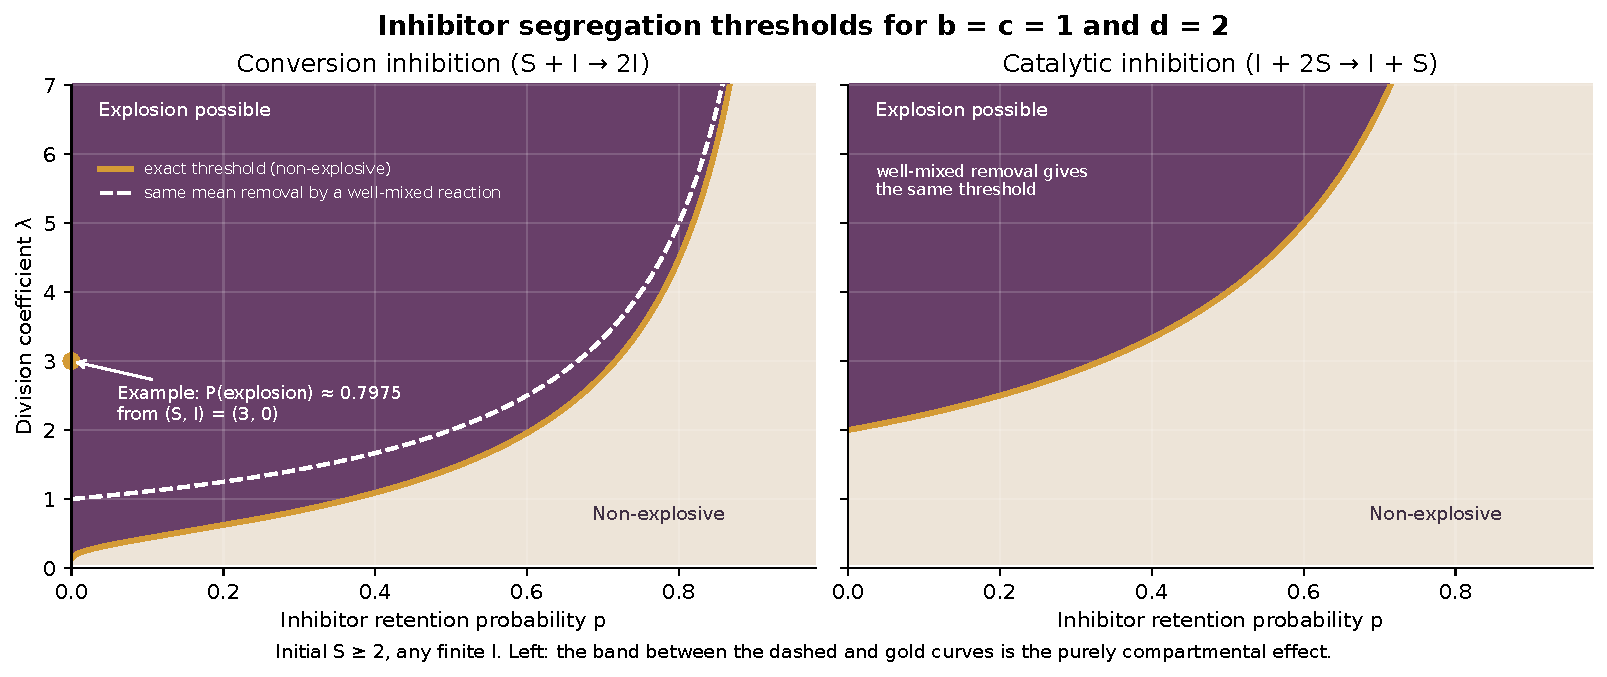
\includegraphics[width=\linewidth]{phase_diagram.pdf}
\caption{Exact phase boundaries for $b=c=1$, $d=2$ and fixed retention $Q\equiv p$. Purple: explosion with positive probability. Gold curve: the boundary, which is nonexplosive. Left, conversion inhibition: the dashed curve is the threshold $\lambda(1-p)=d-b$ for the well-mixed reaction $S+I\to S$ that removes the same mean amount of inhibitor; the band between the curves is the purely compartmental effect of bulk export. Right, catalytic inhibition: the two thresholds coincide. The dot marks the example of Section~\ref{sec:example}.}\label{fig:phase}
\end{figure}

\subsection{Why it happens}\label{sec:mechanism}
The proofs rest on one change of clock. Run time at speed $S$, that is, use the operational time $u$ with $du=S\,dt$. In this clock the inhibitor evolves on its own: it is a branching (conversion) or immigration (catalysis) process hit by random \emph{catastrophes}, the divisions, at rate $\lambda$, each of which thins it. The substrate, in the same clock, grows like a Yule process at rate $b$ and loses one molecule at each inhibition event. Explosion happens exactly when the substrate wins this race, because once the substrate grows exponentially in operational time, the physical time $\int du/S$ needed for infinitely many events is finite.

In the conversion family each inhibitor reproduces. Repeated thinning by a factor $Q$ at rate $\lambda$ changes its growth exponent from $d$ to $d+\lambda\E\log Q$, a standard fact about branching under catastrophes \cite{KaplanSudburyNilsen1975,HermannPfaffelhuber2020}. The substrate wins when this exponent is below $b$. The logarithm is the signature of bulk removal: a well-mixed degradation reaction with the same mean effect changes the exponent only to $d-\lambda(1-\E Q)$, which is larger. In the catalytic family the inhibitor does not reproduce, only its long-run average $c/(\lambda(1-\E Q))$ matters, and bulk and per-molecule removal give the same threshold.

\subsection{What is new and what is classical}\label{sec:contribution}
Every probabilistic ingredient is known, and we cite each at the point of use:
\begin{itemize}
\item linear birth--death processes in a time-varying environment and their generating functions \cite{Kendall1948,BacaerEdDarraz2014};
\item immigration and branching processes with binomial catastrophes \cite{BrockwellGaniResnick1982,Economou2004,KapodistriaPhungDucResing2016,BenAriRoitershteinSchinazi2019,GalloRoldanCorrea2026};
\item survival thresholds of branching under disasters, including the logarithmic criterion and random retention \cite{KaplanSudburyNilsen1975,BansayePardoSmadi2013,HermannPfaffelhuber2020};
\item Yule populations with scheduled removals triggered by another process, and their summability criterion \cite{LeskelaRobertSimatos2009}, together with related emigration models \cite{Pakes1989,Braun2022};
\item the order-duality viewpoint behind our Poisson-binomial identity \cite{Siegmund1976,AsmussenSigman1996}, and predator--prey growth comparisons \cite{Coffey1995}.
\end{itemize}
The candidate contribution is the chemical construction within the framework of \cite{AHRLL2026}, its exact reduction to these objects, and the resulting sharp classification within each of the two parametric families, with the exact laws and comparisons above. A bounded literature search (Section~\ref{sec:scope}) did not find these chemical embeddings; that does not establish priority.

A companion release \cite{EP2026companion} treats the opposite question raised by the same source paper \cite[Conjecture~3.14]{AHRLL2026}: when division \emph{prevents} explosion of a superlinear producer whose catalysts are conserved. There, too, a logarithmic retention loss $\E[-\log Q]$ sets a critical boundary. The two results are complementary: in \cite{EP2026companion} dilution of the \emph{growing} species stabilises, while here export of the \emph{inhibiting} species destabilises.

\subsection{Reading guide}
Section~\ref{sec:model} fixes the model and proves the general reduction to a single active compartment. Section~\ref{sec:conversion} proves the conversion results, Section~\ref{sec:catalytic} the catalytic ones, and Section~\ref{sec:randomQ} extends both to random retention. Section~\ref{sec:compare} contains the comparison with well-mixed removal and continuity at threshold. Section~\ref{sec:numerics} gives the quantitative computations and Section~\ref{sec:scope} the scope and limitations. Each section opens with a plain-language summary. Table~\ref{tab:notation} collects notation.

\begin{table}[ht]
\centering\small
\caption{Notation.}\label{tab:notation}
\begin{tabular}{@{}ll@{}}
\toprule
$s,i$; $S,I$ & substrate and inhibitor counts in the active compartment\\
$b,c,d$ & autocatalysis, inhibitor-production and inhibition coefficients\\
$\lambda$; $p$ or $Q$ & division coefficient; inhibitor retention probability at a division\\
$u$, $t(u)$ & operational time ($du=S\,dt$) and the corresponding physical time\\
$Z=S-1$ & substrate excess over one molecule\\
$N_\lambda$, $N_c$ & Poisson processes of divisions and of inhibitor production, in operational time\\
$D$, $\tau_j$ & point process and times of inhibitor births (conversion events)\\
$\gamma=d+\lambda\E\log Q$ & growth exponent of the thinned inhibitor population (conversion)\\
$\mu$, $r=b-d\mu$ & mean inhibitor level and substrate growth exponent (catalysis)\\
$T$ & explosion time ($T=\infty$ if no explosion); $C(t)$ number of compartments\\
\bottomrule
\end{tabular}
\end{table}
\section{The model and a general reduction}\label{sec:model}
\takeaway{When every reaction needs the substrate and the substrate never leaves the active compartment, the whole population of compartments behaves like a single compartment that occasionally throws away some inhibitor. A change of clock then separates the inhibitor from the substrate.}

\subsection{The compartment framework}\label{sec:framework}
We use the framework of \cite[\S2.2]{AHRLL2026}, specialised to no inflow, exit or coagulation. A chemistry with $m$ species is a finite set of reactions $\nu\to\nu'$ with $\nu,\nu'\in\Z_{\ge0}^m$ and propensities $\lambda_{\nu\to\nu'}(x)$. The state of the compartment model is a finitely supported function $n:\Z_{\ge0}^m\to\Z_{\ge0}$, where $n_x$ counts compartments with contents $x$; the zero vector is an admissible content, so empty compartments are retained and counted, and the total number of compartments is $C(n)=\sum_xn_x$. Each compartment reacts independently with the given propensities. A compartment with contents $x$ divides at rate $\lambda S(x)$, where $S(x)$ is its count of the designated species $S$, and is replaced by daughters with contents $y$ and $x-y$, where $y$ is drawn from a fixed probability law $\psi(x,\cdot)$ supported on $0\le y\le x$ \cite[\S2.2]{AHRLL2026}. The source framework allows any such mass-conserving $\psi$; its own examples include independent fair allocation of every molecule.

Throughout, the process is the minimal continuous-time Markov chain with these rates, and its \emph{explosion time} $T\in(0,\infty]$ is the limit of its jump times. The process is \emph{nonexplosive} from a state if $T=\infty$ almost surely. Every division counts as an event, including one whose second daughter is empty.

\begin{definition}[Selective segregation]\label{def:selective}
A kernel $\psi$ is \emph{substrate-keeping} if one daughter receives every $S$ molecule. For the two-species chemistries of this paper, with contents $(s,i)$, the \emph{inhibitor-segregation kernel with retention law $\mathcal L(Q)$} sends $(s,i)$ to $(s,K)$ and $(0,i-K)$, where, conditional on $Q\sim\mathcal L(Q)$, $K\sim\Bin(i,Q)$. Fixed retention $Q\equiv p$ is the special case $\mathcal L(Q)=\delta_p$.
\end{definition}

This kernel is mass-conserving and fixed for each parent state (its daughter law is the mixture $\E\Bin(i,Q)$), so it is admissible in \cite{AHRLL2026}; drawing $Q$ afresh at each division is the same thing as using this mixture kernel. It is not exchangeable between species: it treats $S$ and $I$ differently. Section~\ref{sec:scope} discusses what is and is not known for kernels that do not distinguish species.

\subsection{The two chemistries}
Both chemistries have species $S$ and $I$ and the reactions listed in Table~\ref{tab:results}. We write propensities as functions of $(s,i)$; in the binomial-coefficient convention of \cite{AHRLL2026} the rate constants are $2b,c,d$ (conversion) and $2b,c,2d$ (catalysis). No reaction has an empty source complex, and the conversion chemistry has at most two reactant molecules per reaction. These facts do not make the chemistry mass-conserving: $2S\to3S$ and $S\to S+I$ are open-resource production reactions, as is standard in reaction-network models. The phrase ``no inflow'' is meaningful in the sense of Observation~3.7 of \cite{AHRLL2026}: no reaction runs faster in pieces than in bulk.

\subsection{Reduction to one active compartment}
\begin{proposition}[Single-lineage reduction]\label{prop:reduction}
Suppose every reaction of the chemistry has $S$ in its source complex and $\psi$ is substrate-keeping. Start from one compartment with contents $x_0$. Then:
\begin{enumerate}[label=(\alph*)]
\item compartments with no $S$ are inert: they never react or divide;
\item at every time before explosion there is exactly one compartment containing $S$ (the \emph{active} compartment), or none, and its contents $X(t)$ form a continuous-time Markov chain with the chemical transitions together with the \emph{export} transitions $x\mapsto z$ at rate $\lambda S(x)\widehat\psi(x,z)$, $z\ne x$, where $\widehat\psi(x,z)=\psi(x,z)+\psi(x,x-z)$ for $S(z)=S(x)$ is the law of the substrate-containing daughter;
\item the compartment model explodes if and only if $X$ explodes, and the explosion times agree.
\end{enumerate}
For several initial compartments, the active descendants of different initial compartments evolve independently, and the model explodes if and only if one of them does.
\end{proposition}

\begin{proof}
(a) An $S$-free compartment has every propensity equal to zero, since each source complex contains $S$, and division rate $\lambda S(x)=0$. (b) A division of the active compartment produces one daughter with all of its $S$ and one $S$-free, hence inert, daughter. Reactions never create $S$ in an $S$-free compartment. So the active compartment is unique; whichever daughter receives the substrate, its contents have law $\widehat\psi(x,\cdot)$, and $X$ jumps as stated. A division whose substrate daughter equals the parent leaves $X$ unchanged but still adds an empty compartment. (c) Every event of the compartment model is either a jump of $X$ or such a silent division. The latter occur at rate at most $\lambda S(X)$. If $X$ makes finitely many jumps on $[0,t]$, then $S(X)$ is bounded on $[0,t]$ and these silent divisions are finitely many there, almost surely. Conversely, explosion of $X$ is explosion of the full model. The statement for several compartments follows because there is no coagulation and no shared inflow.
\end{proof}

\begin{remark}\label{rem:mass-action-emulation}
Proposition~\ref{prop:reduction} says that, under substrate-keeping kernels, compartmentalisation is equivalent to adding to the single-compartment chain a non-mass-action export transition at rate $\lambda s$. The interesting question is therefore how such bulk export compares with an ordinary chemical removal reaction. Section~\ref{sec:compare} answers this exactly for both families.
\end{remark}

\subsection{Operational time}\label{sec:optime}
For both chemistries the active contents are $(S,I)$ with $S\ge1$ until $S$ first hits $0$ (conversion) or forever (catalysis). Divide every physical rate by $S$. Table~\ref{tab:optime} lists the resulting operational-time rates; here $Z=S-1$, and a \emph{division} is a thinning $I\mapsto\Bin(I,Q)$.

\begin{table}[ht]
\centering\small
\caption{Operational-time rates, obtained by dividing physical propensities by $S$.}\label{tab:optime}
\begin{tabular}{@{}lll@{}}
\toprule
Event & Conversion & Catalysis\\
\midrule
$Z\mapsto Z+1$ & $bZ$ & $bZ$\\
$I\mapsto I+1$ (production) & $c$ & $c$\\
inhibition & $(Z,I)\mapsto(Z-1,I+1)$ at rate $dI$ & $Z\mapsto Z-1$ at rate $dIZ$\\
division & $I\mapsto\Bin(I,Q)$ at rate $\lambda$ & $I\mapsto\Bin(I,Q)$ at rate $\lambda$\\
\bottomrule
\end{tabular}
\end{table}

In both columns the inhibitor rates do not involve $Z$. This is the structural fact behind everything that follows.

\begin{lemma}[Graphical construction and time change]\label{lem:timechange}
Let $\mathcal N_c,\mathcal N_\lambda$ be Poisson processes of rates $c,\lambda$ (production and division clocks), let each inhibitor carry its own rate-$d$ birth clock (conversion only), and let thinning decisions use independent uniform marks; let $\mathcal N_b$ and $\mathcal N_{\rm d}$ be independent Poisson random measures on $[0,\infty)^2$, independent of the former, driving substrate births and (catalysis only) substrate deaths. Call the \emph{marked environment} $\mathcal E$ the inhibitor path together with the type of each of its events; in particular $\mathcal E$ contains the point process $D$ of conversion (inhibitor birth) times, which production events do not belong to.
\begin{enumerate}[label=(\alph*)]
\item $\mathcal E$ is a measurable function of the inhibitor clocks and marks alone, the inhibitor process is nonexplosive, and in the conversion case $D$ has intensity $dI(u)$.
\item Given $\mathcal E$, $Z$ is the unique solution of the operational-time equations driven by $\mathcal N_b$ (births at rate $bZ$) and, in the conversion case, by a unit removal at every point of $D$ while $Z>0$, or, in the catalytic case, by $\mathcal N_{\rm d}$ (deaths at rate $dI(u)Z$). It is absorbed at $Z=0$ and nonexplosive on bounded operational intervals.
\item Let $u_0=\inf\{u:Z(u)=0\}\in(0,\infty]$, $t(u)=\int_0^u dv/(Z(v)+1)$ for $u<u_0$ and $T^*=t(u_0-)$. With $u(t)$ the inverse of $t$, the process $(S,I)(u(t))$, $t<T^*$, has the law of the minimal physical-time active chain up to the first time $S=1$. If $u_0=\infty$ and $T^*<\infty$, the physical chain explodes at $T=T^*$; if $u_0=\infty$ and $T^*=\infty$ it is nonexplosive; and if $u_0<\infty$ it is nonexplosive.
\end{enumerate}
The inhibitor process is autonomous: it drives the substrate but is not influenced by it. It is not independent of the substrate path.
\end{lemma}

\begin{proof}
(a) The inhibitor rates in Table~\ref{tab:optime} do not depend on $Z$, so the usual Poisson construction defines $\mathcal E$ pathwise. It is nonexplosive because $I$ is dominated by an immigration--Yule process of rates $c$ and $d$ (conversion) or by $i_0+\mathcal N_c$ (catalysis), and divisions only remove inhibitors. (b) Given $\mathcal E$, the substrate equation is linear, driven by $\mathcal N_b$ and by deterministic removal times (conversion) or by $\mathcal N_{\rm d}$ with a death rate that is bounded on compact intervals (catalysis); it has a unique solution, dominated by a Yule process. (c) Up to $u_0$ the chain $(Z,I)$ jumps with the rates of Table~\ref{tab:optime}, which are the physical rates divided by $S=Z+1\ge1$; the standard random time change for Markov jump processes (for example \cite[Chapter~6]{EthierKurtz1986}) shows that $(Z,I)(u(t))$ is the minimal chain with the physical rates up to $T^*$. If $u_0=\infty$ and $T^*<\infty$, infinitely many operational events, hence physical events, occur before $T^*$, which is therefore the explosion time. If $u_0=\infty$ and $T^*=\infty$, every bounded physical interval corresponds to a bounded operational interval and contains finitely many events. If $u_0<\infty$, then $S=1$ at physical time $T^*<\infty$ and $S\le1$ afterwards, the autocatalytic rate vanishes and $S$ can never increase again; in the conversion case the last substrate molecule may later be converted, after which the compartment is inert. All remaining physical rates are bounded on bounded intervals, so no explosion occurs.
\end{proof}

\takeaway{After the change of clock, the inhibitor is a self-contained random environment, and the substrate is a linear population living in it. Explosion is exactly the event that the substrate grows fast enough in operational time for $\int du/S$ to be finite.}
\section{Conversion inhibition}\label{sec:conversion}
\takeaway{The inhibitor multiplies through conversion and is thinned at each division. If its thinned growth exponent $d+\lambda\log p$ stays below the substrate's exponent $b$, the substrate can outrun it and explode; otherwise the inhibitor wins and the substrate dies out. Conditional on the inhibitor's history, the chance of explosion is an explicit coin-tossing probability.}

\subsection{Statement}
Take $b,c,d,\lambda>0$ with $d>b$, fixed retention $p\in[0,1]$, and one initial compartment with finite contents $(s_0,i_0)$. For $0<p\le1$ put
\[
\gamma=d+\lambda\log p,
\]
and set $\gamma=-\infty$ when $p=0$. Let $\tau_1<\tau_2<\cdots$ be the inhibitor birth (conversion) times of the operational-time inhibitor process of Lemma~\ref{lem:timechange}, extended past the death of the substrate.

\begin{theorem}[Sharp phase boundary for conversion inhibition]\label{thm:conversion}
\leavevmode
\begin{enumerate}[label=(\alph*)]
\item The chemistry without compartments is nonexplosive from every finite state, and its substrate reaches zero almost surely.
\item If $s_0\le1$, the compartment model is nonexplosive.
\item If $s_0\ge2$ and $p=0$, the model explodes with positive probability, for every $\lambda>0$.
\item If $s_0\ge2$ and $0<p<1$, the model explodes with positive probability if and only if
\begin{equation}\label{eq:conv-threshold}
d+\lambda\log p<b,\qquad\text{equivalently}\qquad p<p_c:=\exp\Bigl(-\frac{d-b}{\lambda}\Bigr).
\end{equation}
If $\gamma\ge b$, including equality, the model is nonexplosive and its substrate reaches zero almost surely.
\item If $p=1$ the model is nonexplosive.
\item (Exact conditional law.) Let $z=s_0-1\ge1$. Conditional on the marked environment $\mathcal E$ of Lemma~\ref{lem:timechange}, let $B_1,B_2,\dots$ be independent with $B_j\sim\Ber(e^{-b\tau_j})$ and put $K_\infty=\sum_jB_j\in[0,\infty]$. Then
\begin{equation}\label{eq:PB}
\P(T<\infty\mid\mathcal E)=\P(K_\infty<z\mid\mathcal E);\quad\text{for } s_0=2,\quad \P(T<\infty\mid\mathcal E)=\prod_j\bigl(1-e^{-b\tau_j}\bigr).
\end{equation}
\end{enumerate}
In every explosive case $\P(T<\infty)<1$. Neither $c$ nor $i_0$ affects the phase boundary.
\end{theorem}

The variables $B_j$ live on an extension of the probability space and describe a conditional law; they are not claimed to be functions of the substrate path. Since $\log p\le p-1$, the following explicit region lies strictly inside \eqref{eq:conv-threshold}.

\begin{theorem}[Explicit lower bound]\label{thm:bound}
Let $z=s_0-1\ge1$. If $\Delta:=b+\lambda(1-p)-d>0$, put $K=d(i_0+c/b)/\Delta$. Then
\[
\P(T<\infty)\ \ge\ \max\Bigl\{0,\ 1-\frac Kz\Bigr\}.
\]
For $b=c=1$, $d=2$, $\lambda=3$, $p=0$ and $(s_0,i_0)=(3,0)$ this gives $\Delta=2$, $K=1$, $z=2$ and $\P(T<\infty)\ge1/2$.
\end{theorem}

\begin{theorem}[Blow-up on explosion]\label{thm:asymp-conv}
Under the assumptions of Theorem~\ref{thm:conversion}, almost surely on $\{T<\infty\}$,
\[
(T-t)\,S(t)\longrightarrow\frac1b,\qquad \frac{C(t)}{\log\frac1{T-t}}\longrightarrow\frac\lambda b,\qquad \frac{I_{\rm tot}(t)}{S(t)}\longrightarrow0\qquad(t\uparrow T),
\]
where $C(t)$ is the number of compartments and $I_{\rm tot}(t)$ the number of inhibitor molecules in all compartments.
\end{theorem}

The proofs occupy the rest of this section. Section~\ref{sec:sched} isolates the substrate's behaviour for a fixed schedule of losses. Sections~\ref{sec:upper}--\ref{sec:explosive} prove explosion below the threshold, and Sections~\ref{sec:immigrant}--\ref{sec:nonexplosive} prove nonexplosion at and above it.

\subsection{A Yule population with scheduled removals}\label{sec:sched}
By Lemma~\ref{lem:timechange}, conditional on the marked environment $\mathcal E$, $Z=S-1$ is a Yule process of rate $b$ that loses one individual at each time $\tau_j$ while positive, absorbed at $0$. This object, a Yule population culled at the times of another process, was studied by Leskel\"a, Robert and Simatos \cite[Section~3]{LeskelaRobertSimatos2009} (published as \cite{LeskelaRobertSimatos2010}): their Proposition~3.4 gives positive survival when $\sum_je^{-b\tau_j}<\infty$, and the following paragraph there announces almost sure extinction in the divergent case. We need an exact version.

For $0<q\le1$ let $g_q(s)=qs/(1-(1-q)s)$ be the generating function of $\Geo(q)$ on $\{1,2,\dots\}$. A Yule process of rate $b$ started from one individual is $\Geo(e^{-bu})$ at time $u$, and $g_q\circ g_r=g_{qr}$.

\begin{lemma}[Scheduled removals]\label{lem:sched}
Let $0<\tau_1\le\tau_2\le\cdots$ be a deterministic, locally finite (possibly finite or empty) schedule, let $Z$ start from $z\ge1$, and put $q(u)=e^{-bu}$, $q_j=e^{-b\tau_j}$. Let $B_j\sim\Ber(q_j)$ be independent, $K_u=\sum_{\tau_j\le u}B_j$ and $J_u=(z-K_u)_+$. Then
\begin{enumerate}[label=(\alph*)]
\item $\E s^{Z(u)}=\E\,g_{q(u)}(s)^{J_u}$ for $0\le s\le1$; that is, $Z(u)$ is a sum of $J_u$ independent $\Geo(q(u))$ variables;
\item $\P(Z(u)>0\ \forall u)=\P(K_\infty<z)$, which is positive if $L:=\sum_jq_j<\infty$ and zero if $L=\infty$;
\item $W(u)=e^{-bu}Z(u)$ converges almost surely to a limit $W$ with $\E e^{-\theta W}=\E(1+\theta)^{-J_\infty}$; conditional on $J_\infty=k$, $W$ is $\mathrm{Gamma}(k,1)$, and $\{W>0\}$ coincides up to a null set with survival.
\end{enumerate}
\end{lemma}

\begin{proof}
(a) Represent the $z$ initial individuals as $z$ labelled Yule families and, at each removal time, remove one individual from the lowest-labelled surviving family. This produces the required dynamics, whatever labelling is used. A $\Geo(q)$ family losing one individual dies with probability $q$; otherwise, by memorylessness, the remainder is again $\Geo(q)$. Inductively, conditional on the extinction indicators so far, the surviving families at time $u$ are independent $\Geo(q(u))$ variables: between removals this follows from $g_q\circ g_r=g_{qr}$, and at removal $j$ the indicator that a family dies is a fresh $\Ber(q_j)$ independent of the past indicators. Once all families are gone, extend the indicators by independent coins, which have no effect. This gives (a).

(b) $Z(u)>0$ exactly when $K_u<z$, and the events decrease in $u$. If $L<\infty$ then $\P(K_\infty=0)=\prod_j(1-q_j)>0$ because each $q_j<1$; if $L=\infty$ then $K_\infty=\infty$ almost surely by the second Borel--Cantelli lemma.

(c) Births leave $\E W$ unchanged and removals lower it, so $W$ is a nonnegative supermartingale and converges almost surely. Put $s=e^{-\theta q(u)}$ in (a). As $q\downarrow0$, $g_q(e^{-\theta q})\to1/(1+\theta)$, and $J_u\to J_\infty$, so bounded convergence gives $\E e^{-\theta W}=\E(1+\theta)^{-J_\infty}$; the same argument with an extra bounded function of $J_u$ gives the conditional Gamma law. Hence $\P(W>0)=\P(J_\infty>0)=\P(\text{survival})$. Since extinction forces $W=0$, the two events coincide up to a null set.
\end{proof}

\begin{remark}
The identity in (b) is an elementary lemma proved here for completeness. It is related in spirit to the order duality of Siegmund \cite{Siegmund1976} and Asmussen and Sigman \cite{AsmussenSigman1996}, but we do not claim that this exact formula appears there. Numerically, $\P(K_\infty<z)=\sum_{k<z}[x^k]\prod_j(1-q_j+q_jx)$, and truncating the schedule changes this probability by at most the omitted part of $L$.
\end{remark}

\begin{proof}[Proof of Theorem~\ref{thm:conversion}(f)]
By Lemma~\ref{lem:timechange}, explosion is the event that $Z$ never hits zero and $\int_0^\infty du/(Z+1)<\infty$. By Lemma~\ref{lem:sched}(c), on survival $Z(u)=e^{bu}(W+o(1))$ with $W>0$, so the integral is finite. Hence, up to null sets, explosion is survival of $Z$, and Lemma~\ref{lem:sched}(b), applied conditionally on $\mathcal E$, gives \eqref{eq:PB}.
\end{proof}

\subsection{The explicit bound}\label{sec:bound}
\begin{proof}[Proof of Theorem~\ref{thm:bound}]
Let $m(u)=\E I(u)$. The inhibitor generator gives $m'=c+(d-\lambda(1-p))m$, $m(0)=i_0$, so when $\Delta>0$ a Laplace transform gives $\int_0^\infty e^{-bu}m(u)\,du=(i_0+c/b)/\Delta$. The point process $D$ of conversion times has intensity $dI(u)$, so by monotone convergence $\E K_\infty=\E\sum_je^{-b\tau_j}=d\int_0^\infty e^{-bu}m(u)\,du=K$, where the expectation is over the environment and the auxiliary coins jointly. By \eqref{eq:PB} and Markov's inequality, $\P(T<\infty)=\P(K_\infty<z)\ge1-K/z$.
\end{proof}

\subsection{Upper growth of the inhibitor}\label{sec:upper}
\begin{lemma}\label{lem:upper}
Almost surely $\limsup_{u\to\infty}u^{-1}\log(1+I(u))\le\max\{\gamma,0\}$, with the right side equal to $0$ when $p=0$.
\end{lemma}

\begin{proof}
\emph{Case $0<p<1$.} Condition on the division process $N_\lambda$ and put $R(u)=du+(\log p)N_\lambda(u)$, a right-continuous function with $R(u)/u\to\gamma$ almost surely. Evolving the mean between divisions and multiplying it by $p$ at each division gives
\begin{equation}\label{eq:mN}
m_N(u):=\E[I(u)\mid N_\lambda]=i_0e^{R(u)}+c\int_0^ue^{R(u)-R(v)}\,dv.
\end{equation}
For $\varepsilon>0$ there is a finite $C_\varepsilon$ with $|R(u)-\gamma u|\le\varepsilon u+C_\varepsilon$ for all $u$, and substituting into \eqref{eq:mN} gives $\limsup u^{-1}\log(1+m_N(u))\le\max\{\gamma,0\}+2\varepsilon$. Fix $\kappa>\max\{\gamma,0\}$, so that $m_N(n)\le Ce^{\kappa n}$ for integers $n$. On $[n,n+1]$ ignore divisions and dominate $I$ by an immigration--Yule process started at $I(n)$; its terminal value dominates $\sup_{[n,n+1]}I$ and has conditional mean at most $e^dm_N(n)+c(e^d-1)/d$. Markov's inequality at level $e^{(\kappa+\varepsilon)n}$ and the Borel--Cantelli lemma give $\limsup u^{-1}\log(1+I(u))\le\kappa+\varepsilon$ conditionally on almost every division path, hence unconditionally.

\emph{Case $p=0$.} Every division resets $I$ to zero. Choose $q\in(0,1)$ with $qd<\lambda$ and put $V(i)=(i+1)^q$. Concavity gives $(i+2)^q-(i+1)^q\le q(i+1)^{q-1}$, hence $GV(i)\le(qd-\lambda)V(i)+qc+\lambda$. Applying Dynkin's formula to $e^{\kappa u}V(I(u))$ with $\kappa=\lambda-qd$, stopped at the exit time from $\{i\le n\}$, and letting $n\to\infty$ by Fatou's lemma gives $\sup_u\E V(I(u))\le V(i_0)+(qc+\lambda)/\kappa$. On each unit interval, Jensen's inequality and the immigration--Yule domination give $\E(1+\sup_{[n,n+1]}I)^q\le C$, uniformly in $n$. Markov's inequality at level $e^{q\varepsilon n}$ and Borel--Cantelli give the claim. No first moment of the stationary environment is needed, so this holds even when $\lambda\le d$.
\end{proof}

\subsection{Explosion below the threshold}\label{sec:explosive}
\begin{proof}[Proof of Theorem~\ref{thm:conversion}(c) and the explosive half of (d)]
Suppose $p=0$, or $0<p<1$ and $\gamma<b$. By Lemma~\ref{lem:upper}, choosing $\kappa\in(\max\{\gamma,0\},b)$, $I(u)\le Ce^{\kappa u}$ for large $u$, so $A_\infty:=\int_0^\infty de^{-bu}I(u)\,du<\infty$ almost surely. Let $X_t=\int_0^te^{-bu}\,dD(u)$ and $A_t=\int_0^tde^{-bu}I(u)\,du$; $A$ is the continuous compensator of $X$. For $\sigma_n=\inf\{t:A_t\ge n\}$, $\E X_{\sigma_n}=\E A_{\sigma_n}\le n$, so $X_{\sigma_n}<\infty$ almost surely; and $\sigma_n=\infty$ on $\{A_\infty<n\}$. Taking the union over $n$ gives
\[
L=\sum_je^{-b\tau_j}<\infty\qquad\text{almost surely}.
\]
Every $\tau_j>0$, so conditional on the environment the survival probability in Lemma~\ref{lem:sched}(b) is at least $\prod_j(1-e^{-b\tau_j})>0$. Averaging over the environment, $\P(T<\infty)>0$ from every $s_0\ge2$.
\end{proof}

\subsection{A successful inhibitor family}\label{sec:immigrant}
For the nonexplosive half we need a lower bound on inhibitor growth. It comes from one inhibitor family that grows like its mean. That a single family under binomial disasters survives exactly when $d+\lambda\log p>0$ is classical \cite{KaplanSudburyNilsen1975}, \cite[Corollary~2.7]{HermannPfaffelhuber2020}; we need the pathwise form below, including its dependence on the shared division times.

\begin{lemma}[Successful immigrant]\label{lem:immigrant}
Let $0<p<1$ and $\gamma>0$. There are random $K>0$ and $u_0<\infty$ such that, almost surely, $I(u)\ge Ke^{R(u)}$ for all $u\ge u_0$, with $R$ as in Lemma~\ref{lem:upper}.
\end{lemma}

\begin{proof}
Realise the division times as a homogeneous Poisson process $\omega$ on $\mathbb R$, with shift flow $\theta_v$. Consider one inhibitor present at time $v$ and its descendants $Y_v(u)$, which have Yule births at rate $d$ and independent thinning at each division. Conditionally on $\omega$, $Y_v$ has mean $m_v(u)=e^{R(u)-R(v)}$, right-continuous in $u$, and $M_v=Y_v/m_v$ is a martingale with
\begin{equation}\label{eq:M2}
\E[M_v(u)^2\mid\omega]=1+\int_v^u\frac{d}{m_v(w)}\,dw+\sum_{\tau\in(v,u]\cap\omega}\frac{1-p}{m_v(\tau)},
\end{equation}
where at a division time $m_v(\tau)$ is the post-division value: the Yule part contributes $d/m$ per unit time, and a thinning of a family of size $y$ adds variance $p(1-p)y$ while the mean normaliser changes from $m$ to $pm$, adding $(1-p)/(pm)=(1-p)/m_v(\tau)$. Because $\gamma>0$, $m_v$ grows exponentially and the division count grows linearly, so both terms in \eqref{eq:M2} converge. Hence $M_v\to W_v$ in $L^2$ with $\E[W_v\mid\omega]=1$, and the conditional Paley--Zygmund inequality gives
\[
\mathfrak q(\theta_v\omega):=\P(W_v>0\mid\omega)\ \ge\ \frac{1}{\E[W_v^2\mid\omega]}>0 .
\]
The function $\mathfrak q$ is measurable: $\mathfrak q(\omega)=\lim_{k\to\infty}\lim_{n\to\infty}\E[\min\{1,kM_0(n)\}\mid\omega]$ by bounded and then monotone convergence, and each $\E[\min\{1,kM_0(n)\}\mid\omega]$ is an integral, over the independent birth and thinning randomness, of a measurable function of $\omega$ restricted to $[0,n]$. The process $v\mapsto\mathfrak q(\theta_v\omega)$ is jointly measurable and stationary, and the Poisson shift flow is ergodic, so Birkhoff's theorem gives $U^{-1}\int_0^U\mathfrak q(\theta_v\omega)\,dv\to\E\mathfrak q>0$, and therefore $\int_0^\infty\mathfrak q(\theta_v\omega)\,dv=\infty$ almost surely.

Conditional on $\omega$, inhibitors produced by $S\to S+I$ arrive as a Poisson process of rate $c$ and their families are independent. Marking each arrival at time $v$ by the event $\{W_v>0\}$ gives a Poisson process of successful arrivals with intensity $c\,\mathfrak q(\theta_v\omega)$, which has infinitely many points almost surely. Take one, at time $v$. Its family is part of the inhibitor population, so $I(u)\ge Y_v(u)=e^{R(u)-R(v)}(W_v+o(1))$, and $K=\tfrac12e^{-R(v)}W_v$ works.
\end{proof}

\subsection{Nonexplosion at and above the threshold}\label{sec:nonexplosive}
\begin{proof}[Proof of the nonexplosive half of Theorem~\ref{thm:conversion}(d)]
Let $0<p<1$ and $\gamma\ge b>0$. We first show $\limsup_{u\to\infty}e^{-bu}I(u)=\infty$. If $\gamma>b$ this is immediate from Lemma~\ref{lem:immigrant}. If $\gamma=b$, let $X_n$ be the increment of $R(u)-bu$ over $[n-1,n]$ and $S_n=X_1+\dots+X_n$. The $X_n$ are independent, identically distributed and integrable with mean $\gamma-b=0$, and $X_n\le a:=d-b$, with equality when $[n-1,n]$ contains no division, an event of probability $e^{-\lambda}$. For $h>0$ let $\tau_h=\inf\{n:S_n\ge h\}$. Since upward steps are at most $a$, the stopped process $h+a-S_{n\wedge\tau_h}$ is a nonnegative martingale and converges almost surely. On $\{\tau_h=\infty\}$ this forces $S_n$ to converge, and hence $X_n\to0$, which is impossible because $X_n=a$ infinitely often almost surely. So every integer level is reached, and intersecting over countably many levels gives $\sup_nS_n=\infty$, and therefore $\limsup_nS_n=\infty$. Lemma~\ref{lem:immigrant} gives $e^{-bn}I(n)\ge Ke^{S_n}$, so the claim follows.

Now suppose, for contradiction, that $Z$ never hits zero, on an event of positive probability. Then every conversion removes one substrate molecule, so $S(u)=s_0+B_S(u)-D(u)>0$, where $B_S$ counts substrate births. The births occur at rate $b(S-1)\le b(s_0+B_S)$, so $s_0+B_S$ is dominated by a Yule process $Y$ of rate $b$ started at $s_0$, and $e^{-bu}Y(u)$ has a finite limit. Inhibitors are created only by production and conversion and divisions only remove them, so $D(u)\ge I(u)-i_0-N_c(u)$, where $N_c$ grows linearly. Hence $\limsup e^{-bu}D(u)=\infty$, contradicting $D(u)<s_0+B_S(u)\le Y(u)$. So $Z$ hits zero almost surely, and by Lemma~\ref{lem:timechange}(c) the model is nonexplosive. After $Z$ hits zero, $S=1$ and the next conversion, which occurs almost surely because $I$ grows, removes it.
\end{proof}

\subsection{Isolated chemistry and endpoint cases}\label{sec:endpoints}
\begin{proof}[Proof of Theorem~\ref{thm:conversion}(a), (b), (e) and $\P(T<\infty)<1$]
(a) Without divisions, $I$ is an immigration--Yule process with rate $c+dI$ in operational time. After its first production event, one Yule family of rate $d$ has a strictly positive normalised limit, so $I(u)\ge Ke^{du}$ eventually. Since $d>b$, the accounting argument of Section~\ref{sec:nonexplosive} forces $Z$ to hit zero, and the chemistry is nonexplosive. (b) If $s_0\le1$ the autocatalytic rate is zero for ever and Lemma~\ref{lem:timechange}(c) applies. (e) If $p=1$ every division exports nothing, so the active compartment runs the isolated chemistry and Proposition~\ref{prop:reduction}(c) applies. Finally, with positive probability the environment has at least $z$ conversion events in $[0,1]$, and on that event $\P(K_\infty\ge z\mid\mathcal E)\ge\prod_{j\le z}e^{-b\tau_j}\ge e^{-bz}>0$; so $\P(T<\infty)<1$.
\end{proof}

\subsection{Blow-up asymptotics}\label{sec:asymp}
\begin{proof}[Proof of Theorem~\ref{thm:asymp-conv}]
By Section~\ref{sec:sched}, up to null sets the explosion event is $\{W>0\}$, on which $S(t(u))=Z(u)+1=e^{bu}(W+o(1))$. Fix $\varepsilon\in(0,W)$; for large $v$, $W-\varepsilon\le e^{-bv}Z(v)\le W+\varepsilon$, so $T-t(u)=\int_u^\infty dv/(Z(v)+1)$ lies between $e^{-bu}/(b(W\pm\varepsilon))$ up to factors tending to one. Letting $\varepsilon\to0$ gives $T-t(u)\sim e^{-bu}/(bW)$, hence $(T-t(u))S(t(u))\to1/b$. Each division adds one compartment, so $C(t(u))=1+N_\lambda(u)\sim\lambda u$, while $\log(1/(T-t(u)))\sim bu$. Since $u\mapsto t(u)$ is a continuous increasing bijection of $[0,\infty)$ onto $[0,T)$, these limits hold as $t\uparrow T$. For the composition, divisions conserve $I_{\rm tot}$ and each production or conversion adds one inhibitor, so $I_{\rm tot}(t(u))=i_0+N_c(u)+D(u)$. On $\{W>0\}$ we have $L=\sum_je^{-b\tau_j}<\infty$ (otherwise $Z$ dies by Lemma~\ref{lem:sched}(b)), so $e^{-bu}D(u)=\sum_{\tau_j\le u}e^{-b\tau_j}e^{-b(u-\tau_j)}\to0$ by dominated convergence. As $N_c$ grows linearly and $S(t(u))\sim We^{bu}$, $I_{\rm tot}/S\to0$.
\end{proof}
\section{Catalytic inhibition}\label{sec:catalytic}
\takeaway{Here the inhibitor does not reproduce; it is produced and exported. Its long-run average level is $\mu=c/(\lambda(1-p))$, and the substrate's growth exponent in operational time is $r=b-d\mu$. Explosion is possible exactly when $r>0$, and conditional on the inhibitor's history its probability has a closed form.}

\subsection{Statement}
Take $b,c,d,\lambda>0$, $p\in[0,1]$ and one initial compartment $(s_0,i_0)$. For $p<1$ put
\[
\mu=\frac{c}{\lambda(1-p)},\qquad r=b-d\mu .
\]
In operational time (Table~\ref{tab:optime}) the inhibitor $I$ is an immigration process with binomial catastrophes; it is autonomous, that is, constructed from its own clocks and not influenced by $Z$. Given its path, put $R(u)=bu-d\int_0^uI(v)\,dv$ and $D_u=\int_0^ue^{-R(v)}\,dv$.

\begin{theorem}[Catalytic inhibition]\label{thm:catalytic}
\leavevmode
\begin{enumerate}[label=(\alph*)]
\item The chemistry without compartments is nonexplosive from every finite state.
\item If $s_0\le1$ the compartment model is nonexplosive for every $p$; if $p=1$ it is nonexplosive.
\item If $s_0\ge2$ and $0\le p<1$, the model explodes with positive probability if and only if $r>0$, that is
\begin{equation}\label{eq:cat-threshold}
b\lambda(1-p)>dc,\qquad\text{equivalently}\qquad p<p_c^{\rm cat}:=1-\frac{dc}{b\lambda}.
\end{equation}
If $r\le0$, including equality, it is nonexplosive.
\item In the supercritical case explosion coincides, up to null sets, with survival of $Z$, and almost surely on $\{T<\infty\}$
\[
\frac{\log S(t)}{\log\frac1{T-t}}\to1,\qquad \frac{C(t)}{\log\frac1{T-t}}\to\frac\lambda r,\qquad\frac{I_{\rm tot}(t)}{\log\frac1{T-t}}\to\frac cr .
\]
\item (Exact conditional law.) If $r>0$ and $s_0\ge2$, then $D_\infty<\infty$ almost surely and
\begin{equation}\label{eq:cat-law}
\P(T<\infty\mid I)=1-\Bigl(1-\frac1{bD_\infty}\Bigr)^{s_0-1}\in(0,1).
\end{equation}
\end{enumerate}
\end{theorem}

\subsection{Regeneration of the inhibitor environment}\label{sec:regen}
For $0\le p<1$ the inhibitor has generator $Gf(i)=c[f(i+1)-f(i)]+\lambda\{\E f(\Bin(i,p))-f(i)\}$. This immigration--catastrophe chain and its stationary law are classical \cite{BrockwellGaniResnick1982,Economou2004,BenAriRoitershteinSchinazi2019}; for completeness we prove the two facts we use. A \emph{cycle} starts on entry to $0$, includes the holding time there until the next production event, and ends at the next return to $0$; cycles are independent and identically distributed.

\begin{lemma}\label{lem:cycles}
The cycle length $\tau$ has an exponential moment, the cycle reward $A=\int_0^\tau I(u)\,du$ has moments of all orders, and $c\,\E\tau=\lambda(1-p)\E A$. Consequently $u^{-1}\int_0^uI(v)\,dv\to\mu$ almost surely from every finite initial state.
\end{lemma}

\begin{proof}
Sample $I$ at all points of the superposition of the production and division clocks, a Poisson process of rate $q=c+\lambda$; this \emph{uniformised} chain $Y_n$ includes silent divisions and is not the jump chain. With $a=1+\lambda/(2c)$, $V(i)=a^i$ and $h=p+(1-p)/a<1$,
\[
\frac{\E[V(Y_{n+1})\mid Y_n=i]}{V(i)}=\frac{ca+\lambda h^i}{c+\lambda}.
\]
Choose $K\ge1$ with $h^K\le1/4$; then for $i\ge K$ the ratio is at most $\rho=(c+3\lambda/4)/(c+\lambda)<1$. For the hitting time $\tau_F$ of $F=\{0,\dots,K-1\}$, the stopped supermartingale $\rho^{-n}V(Y_n)$ and Fatou's lemma give $\E_i\rho^{-\tau_F}\le a^i$. From any state in $F$ the next step reaches $0$ with probability at least $\varepsilon=\frac{\lambda}{c+\lambda}(1-p)^{K-1}$; if it does not, the chain is at a state $\le K$ and returns to $F$ after a time $R$ with $\E\rho^{-R}\le a^K$. As $\theta\downarrow0$, $\E_x[e^{\theta(1+R)};\text{failure}]\to\P_x(\text{failure})\le1-\varepsilon$ by dominated convergence (dominated by $\rho^{-1-R}$), uniformly over the finitely many $x\in F$, so for small $\theta>0$ these are at most $1-\varepsilon/2$. The strong Markov property then bounds $\E e^{\theta N}$ by a convergent geometric series, where $N$ is the number of uniformised steps to reach $0$. Holding times are independent $\Exp(q)$, so $\E e^{\eta\tau_0}=\E(q/(q-\eta))^N<\infty$ for small $\eta>0$. At $0$ the time to the next production is $\Exp(c)$ (divisions there are silent), so $\tau$ has an exponential moment.

During a cycle $I(u)\le N_c(u)$, so $A\le\tau N_c(\tau)$, and $\P(N_c(\tau)>x)\le\P(\tau>x/(2c))+\P(\mathrm{Poisson}(x/2)>x)$ decays exponentially; no independence between $\tau$ and $N_c$ is needed. Since $GI(i)=c-\lambda(1-p)i$, Dynkin's formula over one cycle, justified by these moments, gives $0=c\E\tau-\lambda(1-p)\E A$, and the renewal-reward theorem gives the limit $\E A/\E\tau=\mu$.
\end{proof}

\subsection{The conditional branching formula}\label{sec:kendall}
Fix an inhibitor path. Given it, $Z$ is a linear birth--death process with birth rate $b$ and time-varying death rate $dI(u)$ per individual. Kendall's formula \cite{Kendall1948} (see also \cite{CogburnTorrez1981,BacaerEdDarraz2014} for random environments) gives, for $Z(0)=1$,
\begin{equation}\label{eq:kendall}
F_u(s):=\E[s^{Z(u)}\mid I]=1-\frac{1-s}{e^{-R(u)}+bD_u(1-s)},\qquad q_u:=\P(Z(u)>0\mid I)=\frac1{e^{-R(u)}+bD_u}.
\end{equation}
To verify it directly, put $\alpha=e^{-R}$ and $\beta=bD$: these are absolutely continuous with $\alpha'=(-b+dI)\alpha$ and $\beta'=b\alpha$ almost everywhere, and \eqref{eq:kendall} satisfies the forward equation $\partial_uF=(s-1)(bs-dI(u))\partial_sF$ for almost every $u$, with $F_0(s)=s$; uniqueness for the integrated equation gives \eqref{eq:kendall}. For $z$ initial individuals the generating function is $F_u(s)^z$. The identity $e^{-R(u)}+bD_u=1+\int_0^udI(v)e^{-R(v)}\,dv\ge1$ shows that all quantities are probabilities. Finally $W_u=e^{-R(u)}Z(u)$ is a nonnegative conditional martingale with mean $z$ and converges almost surely.

\subsection{Proofs}\label{sec:cat-proofs}
\begin{proof}[Proof of Theorem~\ref{thm:catalytic}(c), (d) and (e)]
\emph{Supercritical case.} By Lemma~\ref{lem:cycles}, $R(u)/u\to r$. If $r>0$ then $R\to\infty$ and $D_\infty<\infty$, so $q_\infty=1/(bD_\infty)>0$, and $q_\infty<1$ because $\int_0^\infty dIe^{-R}>0$. Substituting $s=e^{-\theta e^{-R(u)}}$ into \eqref{eq:kendall} and letting $u\to\infty$ gives, for one ancestor, $\E[e^{-\theta W}\mid I]=(1-q_\infty)+q_\infty\cdot q_\infty/(q_\infty+\theta)$: $W$ has an atom $1-q_\infty$ at $0$ and is otherwise exponential. With $z$ ancestors, $\P(W>0\mid I)=1-(1-q_\infty)^z$, which equals the survival probability; since extinction forces $W=0$, survival and $\{W>0\}$ coincide up to null sets. On that event $Z(u)=e^{R(u)}(W+o(1))\ge e^{ru/2}$ for large $u$, so $\int_0^\infty du/(Z+1)<\infty$ and the model explodes by Lemma~\ref{lem:timechange}; on extinction it does not. This proves \eqref{eq:cat-law}.

\emph{Asymptotics.} On $\{W>0\}$, $u^{-1}\log S(t(u))\to r$. Bounding $S(t(v))$ between constant multiples of $e^{(r\pm\varepsilon)v}$ for large $v$ and integrating gives $-u^{-1}\log(T-t(u))\to r$, and combining the two limits gives the first statement of (d). Each division adds a compartment and no inhibitor is destroyed, so $C(t(u))=1+N_\lambda(u)$ and $I_{\rm tot}(t(u))=i_0+N_c(u)$; the strong laws for these Poisson processes give the other two limits. Unlike the conversion family, $(T-t)S(t)$ need not converge here, because the active inhibitor count keeps regenerating.

\emph{Subcritical case.} If $r<0$ then $R\to-\infty$, so $q_u\to0$: $Z$ dies out almost surely and, by Lemma~\ref{lem:timechange}(c), the model is nonexplosive.

\emph{Critical case.} If $r=0$, consider the values of $R$ at the starts of the regeneration cycles after the first visit to $0$. Their increments $Y_n=b\tau_n-dA_n$ are independent, identically distributed, with mean $0$ and finite variance, and the variance is at least $b^2/c^2>0$ because each cycle begins with an independent $\Exp(c)$ holding time at $0$ that contributes $b$ times itself to $Y_n$. The central limit theorem gives $\P(\sum_{k\le n}Y_k<-m)\to1/2$ for each $m$; hence $\liminf_n\sum_{k\le n}Y_k=-\infty$ with probability at least $1/2$, and by the Hewitt--Savage zero--one law with probability one. Since $R'\le b$, $\int_v^{v+1}e^{-R(u)}du\ge e^{-R(v)}(1-e^{-b})/b$, so $D_\infty=\infty$, $q_u\le1/(bD_u)\to0$, and the model is nonexplosive. This includes the boundary $b\lambda(1-p)=dc$.
\end{proof}

\begin{proof}[Proof of Theorem~\ref{thm:catalytic}(a) and (b)]
Without divisions $I(u)=i_0+N_c(u)$, so $u^{-2}\int_0^uI\to c/2$ and $R\to-\infty$ quadratically; $Z$ dies out, after which $S=1$ for ever and only production events occur, at constant physical rate. If $s_0\le1$ the autocatalytic and inhibition rates vanish for ever. If $p=1$ divisions export nothing and Proposition~\ref{prop:reduction}(c) reduces the model to the isolated chemistry.
\end{proof}

\begin{remark}[Explosion is less locked in]\label{rem:cat-fragile}
In the conversion family, on survival the discounted contribution $\sum_{\tau_j>u}e^{-b\tau_j}$ of later removals tends to zero and $(T-t)S(t)\to1/b$. In the catalytic family a large inhibitor excursion late in operational time still multiplies every substrate molecule's death rate. Simulations stopped when the substrate first reaches a level $M$ therefore overestimate the explosion probability noticeably until $M$ is large; for $(b,c,d,\lambda,p)=(2,1,\tfrac12,1,\tfrac12)$ and $s_0=2$, the fraction reaching $M$ fell from about $0.845$ to $0.820$ as $M$ rose from $30$ to $3000$ in an internal check. Numerical estimates for this family should use \eqref{eq:cat-law} with an explicit tail bound, which we do not provide here.
\end{remark}
\section{Random retention at division}\label{sec:randomQ}
\takeaway{If the probability of keeping each inhibitor varies from one division to the next, the conversion threshold depends on the average of $\log Q$, but the catalytic threshold depends only on the average of $Q$. Two division rules with the same average retention can therefore put the conversion chemistry on opposite sides of its threshold.}

Let $Q_1,Q_2,\dots$ be independent copies of a random variable $Q\in[0,1]$ with an arbitrary law, independent of all other randomness, and use $Q_j$ at the $j$th division of the active compartment (Definition~\ref{def:selective}). We interpret $\E\log Q\in[-\infty,0]$ with $\log0=-\infty$. Fresh retention at each catastrophe is an established model for immigration processes \cite{GalloRoldanCorrea2026}, and the logarithmic criterion for branching under random multiplicative catastrophes is classical \cite{BansayePardoSmadi2013,HermannPfaffelhuber2020}. What follows is the consequence for the two chemistries. Retention decisions for different molecules at the same division are independent given $Q_j$ but correlated unconditionally: $\operatorname{Cov}(X_1,X_2)=\Var(Q)$ for the retention indicators $X_1,X_2$ of two molecules. Variability of $Q$ therefore means that inhibitors tend to leave together.

\begin{theorem}[Conversion inhibition with random retention]\label{thm:randomQ-conv}
Assume $d>b$ and $s_0\ge2$. The model explodes with positive probability if and only if
\begin{equation}\label{eq:randomQ-conv}
d+\lambda\,\E\log Q<b ;
\end{equation}
equality is nonexplosive. If $\E\log Q=-\infty$ (for example if $\P(Q=0)>0$) the model explodes with positive probability for every $\lambda>0$. The exact conditional law \eqref{eq:PB} and Theorem~\ref{thm:asymp-conv} hold unchanged, and Theorem~\ref{thm:bound} holds with $\Delta=b+\lambda(1-\E Q)-d$.
\end{theorem}

\begin{proof}
\emph{Finite log-moment.} Suppose $\E|\log Q|<\infty$. Condition on the marked division process and replace $R$ by $R(u)=du+\sum_{j\le N_\lambda(u)}\log Q_j$, whose slope is $\gamma=d+\lambda\E\log Q$ by the strong law for marked Poisson sums. Formula \eqref{eq:mN}, Lemma~\ref{lem:upper} and the explosive half of the proof are unchanged. For Lemma~\ref{lem:immigrant} we need $\gamma>0$, which forces $Q>0$ almost surely; the summand in \eqref{eq:M2} becomes $(1-Q_j)/m_v(\tau_j)\le1/m_v(\tau_j)$, and the measurability and ergodicity argument applies to the marked Poisson flow. The critical argument of Section~\ref{sec:nonexplosive} used only that the increments of $R(u)-bu$ over unit intervals are integrable, independent, identically distributed, centred and bounded above by $a=d-b$, with value $a$ on an event of probability $e^{-\lambda}$; this holds here because $\log Q\le0$. The scheduled-removal lemma depends only on the realised conversion times. The mean equation is $m'=c+(d-\lambda(1-\E Q))m$, which gives the bound.

\emph{Infinite log-moment.} If $\E\log Q=-\infty$, set $Q^\varepsilon=\max\{Q,\varepsilon\}$. By monotone convergence $\E\log Q^\varepsilon\downarrow-\infty$ as $\varepsilon\downarrow0$, so we may choose $\varepsilon$ with $d+\lambda\E\log Q^\varepsilon<b$; the finite case gives $\sum_{\tau\in D^\varepsilon}e^{-b\tau}<\infty$ for the corresponding model. Couple the two inhibitor populations on one labelled graphical construction: common production times; each labelled inhibitor carries one rate-$d$ birth clock, inherited by its offspring labels; and at each division each common molecule uses one uniform mark $U$, being retained in the original model if $U<Q_j$ and in the truncated model if $U<Q_j^\varepsilon$. Since $Q_j\le Q^\varepsilon_j$, the original population is a labelled subset of the truncated one at all times, so every birth time of the original is a birth time of the truncated model, $D\subseteq D^\varepsilon$, and $\sum_{\tau\in D}e^{-b\tau}<\infty$ almost surely. Lemma~\ref{lem:sched} then gives positive explosion probability.
\end{proof}

\begin{theorem}[Catalytic inhibition with random retention]\label{thm:randomQ-cat}
Assume $\P(Q<1)>0$ and put $\mu=c/(\lambda(1-\E Q))$ and $r=b-d\mu$. Theorem~\ref{thm:catalytic} holds with these values; in particular the threshold is
\begin{equation}\label{eq:randomQ-cat}
b\lambda(1-\E Q)>dc ,
\end{equation}
with equality nonexplosive.
\end{theorem}

\begin{proof}
Only Lemma~\ref{lem:cycles} changes. With $w=\P(Q=1)<1$ and $V(i)=a^i$, the uniformised drift ratio is $(ca+\lambda\E[(Q+(1-Q)/a)^i])/(c+\lambda)$, and the expectation tends to $w$ as $i\to\infty$ by dominated convergence. Choosing $a>1$ with $c(a-1)<\lambda(1-w)$ makes the ratio less than one outside a finite set, and from any state in that set a division removes every inhibitor with probability at least a positive constant, because $\E(1-Q)^k>0$ for each $k$. The rest of the proof of Lemma~\ref{lem:cycles} is unchanged, $GI(i)=c-\lambda(1-\E Q)i$ gives the mean, and the critical cycle increments still contain the independent $\Exp(c)$ holding time at zero, so their variance is positive.
\end{proof}

\begin{example}[Same mean retention, different phase]\label{ex:samemean}
Take $b=1$, $d=2$, $\lambda=1$ and any $c>0$. If $Q\equiv\tfrac12$, then $\gamma=2-\log2\approx1.307>1$ and the conversion model is nonexplosive. If $Q=\tfrac1{10}$ or $\tfrac9{10}$ with probability $\tfrac12$ each, then $\E Q=\tfrac12$ but $\gamma=2+\tfrac12\log\tfrac9{100}=2+\log\tfrac3{10}\approx0.796<1$, and the model explodes with positive probability. (The strict inequalities follow from $2<e<3<10/3$.) For the catalytic model both rules give the same threshold. By Jensen's inequality, $\E\log Q\le\log\E Q$, so at fixed mean, variability can only enlarge the explosive region of the conversion model.
\end{example}
\section{What compartments add, monotonicity and robustness}\label{sec:compare}
\takeaway{Division removes inhibitor in bulk at random moments. An ordinary chemical reaction can remove the same average amount continuously. For the self-reproducing inhibitor of the conversion family, bulk removal has a strictly larger explosive region; for the non-reproducing catalytic inhibitor the two give the same threshold. The explosion probability also falls continuously to zero at the threshold, decreases as more inhibitor is kept, and the explosive mechanism survives if each division lets a bounded number of substrate molecules escape.}

\subsection{Bulk export versus well-mixed removal}
Add to the conversion chemistry a well-mixed inhibitor-removal reaction
\begin{equation}\label{eq:degradation}
S+I\longrightarrow S\qquad\text{with propensity }\delta si,\qquad\delta\ge0,
\end{equation}
which removes each inhibitor at rate $\delta$ per unit operational time, and allow divisions with coefficient $\lambda\ge0$ and retention law $Q$ as before ($\lambda=0$ means no compartments). Every reaction still has $S$ in its source complex, so Proposition~\ref{prop:reduction} applies.

\begin{theorem}[Conversion with degradation and division]\label{thm:degradation}
Let $b,c,d>0$, $\delta,\lambda\ge0$ and $s_0\ge2$. The model explodes with positive probability if and only if
\begin{equation}\label{eq:degr-threshold}
d-\delta+\lambda\,\E\log Q<b ,
\end{equation}
and it is nonexplosive at equality; here $\lambda\E\log Q$ is read as $0$ when $\lambda=0$. In particular the well-mixed chemistry with $\lambda=0$ is nonexplosive if and only if $d-\delta\ge b$.
\end{theorem}

\begin{proof}
In operational time the inhibitor now also loses individuals at rate $\delta I$, so it is an immigration--birth--death process with catastrophes; substrate losses are still synchronised with the births alone, and Lemmas~\ref{lem:timechange} and~\ref{lem:sched} apply verbatim. Put $R(u)=(d-\delta)u+\sum_{j\le N_\lambda(u)}\log Q_j$ and $\gamma=d-\delta+\lambda\E\log Q$. Lemma~\ref{lem:upper} holds with this $R$: the conditional mean satisfies $m'=c+(d-\delta)m$ between divisions, the unit-interval domination by an immigration--Yule process ignores deaths, and for $p=0$ the extra term $\delta i[(i)^q-(i+1)^q]$ in $GV$ is nonpositive. The explosive half and the infinite-log-moment coupling are unchanged, each labelled inhibitor now carrying an independent rate-$\delta$ death clock as well as its birth clock.

For the nonexplosive half assume $\gamma\ge b$, so $d>\delta$. In Lemma~\ref{lem:immigrant} the inhibitor families are now linear birth--death processes with rates $d,\delta$, and the integrand in \eqref{eq:M2} becomes $(d+\delta)/m_v$; when $\lambda=0$ or $Q\equiv1$ each family survives with the constant probability $1-\delta/d>0$, and infinitely many families are produced. If $\gamma>b$, or if $\gamma=b$ and divisions genuinely thin ($\lambda>0$, $\P(Q<1)>0$, whence $a=d-\delta-b>0$), the argument of Section~\ref{sec:nonexplosive} applies word for word. In the remaining case $\gamma=d-\delta=b$ without effective divisions, $I(u)\ge Ke^{bu}$ for large $u$, and the accounting bound $D(u)\ge I(u)-i_0-N_c(u)$ still holds because divisions and degradation only remove inhibitors. Integrating by parts,
\[
\int_0^Ue^{-bu}\,dD(u)\ \ge\ b\int_0^Ue^{-bu}D(u)\,du\ \ge\ b\int_{u_0}^U\bigl(K-e^{-bu}(i_0+N_c(u))\bigr)du\ \longrightarrow\ \infty,
\]
so $L=\infty$ and Lemma~\ref{lem:sched}(b) shows that $Z$ dies out almost surely.
\end{proof}

\begin{corollary}[Bulk export is strictly more destabilising]\label{cor:bulk}
Let $d>b$, $\lambda>0$ and $\E Q<1$. Compare
\begin{enumerate}[label=(\roman*)]
\item the compartment model (division coefficient $\lambda$, retention $Q$, $\delta=0$), with
\item the single well-mixed compartment with degradation \eqref{eq:degradation} at $\delta=\lambda(1-\E Q)$ and no divisions.
\end{enumerate}
Both remove each inhibitor at the same mean rate $\lambda(1-\E Q)$ per unit operational time. Model (ii) explodes with positive probability if and only if $\lambda(1-\E Q)>d-b$, and model (i) if and only if $\lambda\,\E\log(1/Q)>d-b$. Since $\log(1/q)\ge1-q$ with equality only at $q=1$, the explosive region of (ii) is strictly contained in that of (i). For $Q\equiv0$, model (i) is explosive for every $\lambda>0$ but model (ii) only for $\lambda>d-b$.
\end{corollary}

The region of model (ii) is exactly the region $\Delta>0$ of Theorem~\ref{thm:bound}: the first-moment bound of Section~\ref{sec:bound} only sees the mean removal rate, which is why it is not sharp for compartments. The band between the two thresholds, shown dashed in Figure~\ref{fig:phase}, is the purely compartmental effect. The logarithm arises because a division removes a random fraction of a whole, self-reproducing population at once: what matters for a multiplicative process is the average of the logarithm of the factor by which it is multiplied, not the average factor.

\begin{proposition}[Catalytic inhibition: bulk and well-mixed removal give the same threshold]\label{prop:massaction}
For the catalytic chemistry with the degradation reaction $S+I\to S$ at propensity $\delta si$, $\delta>0$, and no divisions, the model explodes with positive probability from $s_0\ge2$ if and only if $b\delta>dc$, and is nonexplosive at equality. With $\delta=\lambda(1-\E Q)$ this is exactly the compartment threshold \eqref{eq:randomQ-cat}.
\end{proposition}

\begin{proof}
In operational time the inhibitor is now an immigration--death process (production rate $c$, per-capita death rate $\delta$), autonomous in the sense of Lemma~\ref{lem:timechange}, with mean generator $GI(i)=c-\delta i$. With $V(i)=a^i$ and $a>1$, $GV(i)=a^i[c(a-1)-\delta i(1-1/a)]\le-V(i)$ for $i$ large, so return times to a finite set have exponential moments by the continuous-time Foster--Lyapunov criterion, and from that finite set the chain reaches $0$ within unit time with probability bounded below, so the failed-attempt argument of Lemma~\ref{lem:cycles} gives exponential moments of the cycle length. Lemma~\ref{lem:cycles} therefore holds with $\mu=c/\delta$, and the proofs of Section~\ref{sec:cat-proofs} apply unchanged, including the critical case, where the $\Exp(c)$ holding time at zero again gives positive cycle variance.
\end{proof}

\takeaway{In these two families the purely compartmental effect appears exactly when the exported species reproduces. That is why the conversion threshold involves $\E\log Q$ and the catalytic threshold only $\E Q$. Whether this pattern holds for other chemistries is open.}

\subsection{Monotonicity and continuity at threshold}
\begin{proposition}\label{prop:continuity}
Fix $b,c,d,\lambda>0$, $s_0\ge2$ and $i_0$.
\begin{enumerate}[label=(\alph*)]
\item (Monotonicity.) In both families, if the retention variables can be coupled so that $Q^{(1)}\le Q^{(2)}$ at every division, then the explosion probability with $Q^{(1)}$ is at least that with $Q^{(2)}$. For fixed retention, the explosion probability is nonincreasing in $p$ and nondecreasing in $\lambda$.
\item (Continuity.) For the conversion family with $d>b$, $\P_p(T<\infty)\to0$ as $p\uparrow p_c$. For the catalytic family with $b\lambda>dc$, $\P_p(T<\infty)\to0$ as $p\uparrow p^{\rm cat}_c$.
\end{enumerate}
\end{proposition}

\begin{proof}
Use the labelled graphical construction of Theorem~\ref{thm:randomQ-conv} for all retention laws simultaneously, with a molecule retained at division $j$ when its uniform mark is below $Q_j$. If $Q^{(1)}\le Q^{(2)}$, the first inhibitor population is a labelled subset of the second at all times. For $\lambda$, realise the divisions at rate $\lambda_1$ as a subset of those at rate $\lambda_2>\lambda_1$; extra divisions only remove inhibitors, so the $\lambda_2$ population is a subset of the $\lambda_1$ population.

(a) In the conversion family a smaller inhibitor population has a smaller set of birth times, $D^{(1)}\subseteq D^{(2)}$. The conditional explosion probability $\varphi(D)=\P(\sum_{\tau\in D}B_\tau<z)$ of \eqref{eq:PB} can only decrease when points are added, since each added point carries an extra coin; hence $\varphi(D^{(1)})\ge\varphi(D^{(2)})$, and taking expectations gives the claim. In the catalytic family a smaller inhibitor path gives a larger $R$, a smaller $D_\infty$ and a larger right-hand side in \eqref{eq:cat-law}.

(b) Conversion. As $p\uparrow p_c$ the populations increase. On each interval $[0,u]$ only finitely many marks are used, almost surely none equals $p_c$, so for $p$ close enough to $p_c$ the population on $[0,u]$ coincides with that at $p_c$. Hence $L_p=\sum_{\tau\in D_p}e^{-b\tau}\uparrow L_{p_c}$. At $p_c$ the model is nonexplosive (Theorem~\ref{thm:conversion}(d)), so $\P(K_\infty<z\mid\mathcal E)=0$ almost surely, which by Lemma~\ref{lem:sched}(b) forces $L_{p_c}=\infty$. For independent Bernoulli variables with total mean $L$, $\P(K\le z-1)\le e^{z-1}\E e^{-K}\le\exp\bigl(z-1-(1-e^{-1})L\bigr)$, so $\varphi(D_p)\to0$ and bounded convergence gives $\P_p(T<\infty)\to0$.

Catalysis. In the same way $I_p(v)\uparrow I_{p_c}(v)$ with equality on $[0,u]$ for $p$ near $p_c$, so $e^{-R_p(v)}\uparrow e^{-R_{p_c}(v)}$ for every $v$ and, by monotone convergence, $D_\infty(p)\uparrow D_\infty(p_c)=\infty$ (Section~\ref{sec:cat-proofs}, critical case). Then $1/(bD_\infty(p))\to0$ and \eqref{eq:cat-law} gives $\P_p(T<\infty)\to0$.
\end{proof}

\takeaway{The transition is continuous: just inside the explosive region, explosion is possible but rare. Keeping more inhibitor, or dividing less often, never makes explosion more likely.}

\subsection{Robustness to bounded substrate leakage}
The constructions keep every substrate molecule in one daughter. This can be relaxed for the explosive direction.

\begin{proposition}[Bounded leakage]\label{prop:leakage}
In the conversion family, fix $K\in\N$ and replace the kernel by any mass-conserving kernel under which, from contents $(s,i)$, one marked daughter receives at least $s-K$ substrate molecules and, conditional on $Q$, a $\Bin(i,Q)$ number of inhibitors, the leaked molecules being allocated arbitrarily. If $d+\lambda\E\log Q<b$ and $s_0\ge2$, the model explodes with positive probability.
\end{proposition}

\begin{proof}
Follow the marked lineage, with operational time $du=S_m\,dt$ for its substrate count $S_m$. As before its inhibitor process is autonomous, with production rate $c$, birth rate $dI$ and thinning at rate-$\lambda$ divisions, and $Z_m=S_m-1$ has Yule births at rate $bZ_m$, loses one molecule at each inhibitor birth, and loses at most $K$ at each division time $\sigma_n$. At each division sample the inhibitor thinning first, from its $\Bin(i,Q)$ marginal and with randomness independent of the substrate births, and only then the substrate leak from its conditional law; the times of $D$ and of the divisions $\sigma_n$ then form an autonomous schedule, independent of the substrate birth driver. Work with the killed variable $Z_m=(S_m-1)_+$, stopped when $S_m\le1$. Let $Z'$ have the same births and conversion removals as $Z_m$ but lose exactly $\min\{K,Z'\}$ individuals at each $\sigma_n$, killed at $0$. Order is preserved: births can be coupled monotonically (a Yule process started higher stays higher), a common unit removal preserves $Z'\le Z_m$, and at a division $(x-K)_+\le(y-\ell)_+$ whenever $x\le y$ and $0\le\ell\le K$; hence $Z'\le Z_m$ throughout. The schedule of $Z'$ consists of the times of $D$ together with each $\sigma_n$ repeated $K$ times; it does not depend on the substrate, and its weight $\sum_{D}e^{-b\tau}+K\sum_ne^{-b\sigma_n}$ is finite almost surely, because the first sum is finite as in Section~\ref{sec:explosive} and the second has mean $K\lambda/b$. By Lemma~\ref{lem:sched}, $Z'$ survives and grows like $e^{bu}$ with positive probability; then $S_m\ge Z'+1$, the marked lineage makes infinitely many events in finite physical time, and so does the whole model. Other daughters may contain substrate and be active, but they can only add events.
\end{proof}

The converse direction does not transfer, because leaked substrate can seed new active lineages. Independent splitting of every substrate molecule, as in the fair kernel of \cite{AHRLL2026}, is a different problem (Section~\ref{sec:scope}).
\section{Computing the explosion probability}\label{sec:numerics}
\takeaway{The exact conditional formula turns the explosion probability into an expectation over the inhibitor alone, which never explodes. That expectation can be bounded from both sides by a deterministic computation, or estimated by simulation with explicit error bars.}

Throughout this section we consider the conversion family and write $z=s_0-1$.

\subsection{A two-sided enclosure with controlled rounding}\label{sec:enclosure}
By \eqref{eq:PB}, $\P(T<\infty)=\E\varphi$, where $\varphi=\P(K_\infty<z\mid\mathcal E)$. Attach to the operational inhibitor process a counter $k$ of auxiliary successes: at a conversion at operational time $u$ the counter increases with probability $e^{-bu}$. Then $\P(T<\infty)=f(0,i_0,0)$, where
\[
f(u,i,k)=\P(\text{fewer than $z-k$ further successes after time $u$}\mid I(u)=i)
\]
solves a linear backward equation in $u$ on the states $(i,k)$, $k<z$. We bound $f$ from both sides on a time grid $0=u_0<\dots<u_M=U$ by monotone comparison.
\begin{enumerate}[label=(\roman*)]
\item On $[u_{m-1},u_m]$ the success probability $e^{-bu}$ is replaced by its largest value $e^{-bu_{m-1}}$ for the lower bound and its smallest value $e^{-bu_m}$ for the upper bound; $f$ decreases as success probabilities increase.
\item The inhibitor count is truncated at $N$. Reaching $N+1$ is assigned the payoff $1$ (upper bound) or the first-moment bound $1-\E[\text{further successes}]/(z-k)$ (lower bound), where $\E[\text{further successes}\mid I(u)=i]=d\int_u^\infty e^{-bv}m(v)\,dv$ equals $de^{-bu}(i+c/b)/\Delta$ in the region $\Delta>0$ (for the example, $e^{-u}(i+1)$). The payoff is evaluated at the left end of the step; this is conservative because, at fixed $i$, it increases with $u$.
\item At the horizon $U$ the same payoffs are used.
\item On each step the frozen-rate equation is solved by uniformisation; the omitted Poisson tail is added to the upper bound.
\item Rounding is controlled as follows. Step lengths are powers of two, so grid points, step lengths and Poisson means are exact binary64 numbers. Every exponential, every Poisson weight and tail, and every payoff is computed in decimal arithmetic with 50 significant digits (whose exponential is correctly rounded) and converted to binary64 with a one-unit nudge in the conservative direction; in particular the success probability used for the lower bound is at least $e^{-bu_{m-1}}$. Each decimal quantity is correctly rounded at 50 digits, so its error is far below half a binary64 unit in the last place and the nudged conversion is on the safe side; conversions never go below $0$. A positive payoff $v=1-\E H/(z-k)$ has $\E H/(z-k)<1$ and is therefore computed with absolute error below $10^{-47}$; payoffs below $10^{-20}$, whose unit in the last place could be comparable, are replaced by $0$. All remaining floating-point operations form sums of products of nonnegative numbers; the only subtraction, $1-q$, is exact for $q\ge\frac12$ by Sterbenz's lemma and has relative error at most $2^{-53}$ otherwise. In the standard model each binary64 operation returns the exact result times $(1+e)$ plus $f$, with $|e|\le2^{-53}$ and $|f|<2^{-1074}$ (and $f=0$ for sums). Each operator application and each Poisson-weighted sum (at most $80$ terms) involves at most about ninety successive operations, so its relative error is below $10^{-14}$ and its absolute error far below $10^{-300}$. An outward relative factor $10^{-13}$ and an absolute allowance $10^{-300}$ are applied after every such operation, which also covers underflow. The quantity $\Delta=b+\lambda-d$ is computed exactly as a rational number. The program refuses inputs outside this argument: retention $p\ne0$; rates outside $[1/16,16]$ (which keeps the binary64 uniformisation divisor $\Lambda$ at least $1/16$, so underflow errors stay far below $10^{-300}$ after division; the decimal division by $\Delta$ is unaffected by underflow); $z>10$, $N>2000$ or $U>64$; steps longer than $1/64$; grid points, rates or Poisson means that are not exact binary64 numbers; and more than $80$ Poisson terms.
\end{enumerate}
Each comparison is a coupling of probabilities, and, for the configuration below, the rounding control above makes the computed numbers rigorous bounds, assuming only IEEE-754 binary64 arithmetic with correctly rounded basic operations. The argument is written out here and in the code; it has not been checked by a formal interval-arithmetic library or proof assistant.

For the example of Section~\ref{sec:example} ($b=c=1$, $d=2$, $\lambda=3$, $p=0$, $i_0=0$), with $N=800$, $U=18$ and step $h(u)$ the largest power of two not exceeding $\min\{0.01,5\times10^{-5}e^{u/2}\}$, the computation gives
\[
\begin{array}{lll}
s_0=2: & \P(T<\infty)\in[0.58865,\ 0.58870]\\
s_0=3: & \P(T<\infty)\in[0.79744,\ 0.79751]\\
s_0=4: & \P(T<\infty)\in[0.88702,\ 0.88709]
\end{array}
\]
(outward-rounded). The central value for $s_0=3$ is consistent with the analytic bound $1/2$ and with the simulation estimates below. The script also checks that two corrupted inputs (division coefficient $2.5$ or conversion coefficient $2.25$) and a shifted claimed interval are rejected.

\subsection{An environment-only estimator}\label{sec:estimator}
For a horizon $U$, let $\Phi_U=\P(\sum_{\tau_j\le U}\Ber(e^{-b\tau_j})<z\mid\mathcal E)$, computed by the usual coefficient recursion for Poisson-binomial probabilities. Omitted successes can only reduce survival, so $0\le\E\Phi_U-\P(T<\infty)\le\E\sum_{\tau_j>U}e^{-b\tau_j}$. In the first-moment region $\Delta=b+\lambda(1-\E Q)-d>0$ this is bounded exactly by
\begin{equation}\label{eq:bias}
B_U=\frac{de^{-bU}}{\Delta}\Bigl(m(U)+\frac cb\Bigr),
\end{equation}
by the Laplace-transform calculation of Section~\ref{sec:bound} restarted at $U$. With $n$ independent environment samples and sample mean $\bar\Phi$, Hoeffding's inequality gives, with probability at least $1-\alpha$,
\[
\P(T<\infty)\in\Bigl[\bar\Phi-\sqrt{\log(2/\alpha)/(2n)}-B_U,\ \bar\Phi+\sqrt{\log(2/\alpha)/(2n)}\Bigr].
\]
This error control covers only the region $\Delta>0$; near the sharp boundary a different tail bound would be needed. For the example, $m(U)=1-e^{-U}$, $\Delta=2$ and $B_{10}=2e^{-10}-e^{-20}<9.1\times10^{-5}$. With $n=200{,}000$, $U=10$ and seed $20261028$ the bundled implementation returns $\bar\Phi=0.7967965$ and the 95\% interval $[0.79366,0.79984]$, assuming exact independent sampling; pseudorandom generation and floating-point arithmetic are not verified. Two direct simulations of the full $(S,I)$ chain, which do not use \eqref{eq:PB} and stop once the substrate is large, gave $0.7962\pm0.0013$ and $0.7977\pm0.0009$ (one standard error), both consistent with the enclosure.
\section{Scope, limitations and open questions}\label{sec:scope}

\subsection{Why a nonlinear reaction is needed}
If every source complex has at most one molecule and there are no inflows, the positive chemical drift of the total molecule count $M$ is at most a constant times $M$; division conserves $M$ and creates compartments at rate at most $\lambda M$; so $V=1+C+M$ satisfies $\mathcal LV\le\mathrm{const}\cdot V$ and the model is nonexplosive under every mass-conserving kernel \cite[Theorem~3.1]{AHRLL2026}. The same holds when every source and product complex has at most two molecules, since bimolecular reactions then cannot increase $M$. So quadratic production, with a product complex of three molecules such as $3S$, is the lowest propensity degree at which the present mechanism can operate. We make no minimality claim about numbers of species or reactions.

\subsection{What the result does and does not show}
\begin{itemize}
\item \emph{Selective segregation.} Both constructions use kernels that keep all substrate together (Definition~\ref{def:selective}); Proposition~\ref{prop:leakage} allows a bounded leak. Such kernels are admissible in \cite{AHRLL2026}, so the examples are genuine counterexamples within that framework, but they are an idealisation, not a model of a particular organism. Partitioning at division is known to be a significant source of cell-to-cell variability \cite{HuhPaulsson2011}; we do not claim that any cell partitions an inhibitor in this way.
\item \emph{Molecule-blind division.} For kernels that split every molecule independently, such as the fair kernel of \cite{AHRLL2026}, the substrate is also divided, several compartments stay active, and our reduction fails. Whether Conjecture~3.6 of \cite{AHRLL2026} holds for such kernels without inflow and fusion remains open. The companion classification \cite{EP2026companion} shows that splitting the growing species can by itself prevent explosion, so the answer is likely to depend on a competition between the two effects.
\item \emph{Fragile versus robust nonexplosion.} The isolated conversion chemistry with an extra degradation reaction is nonexplosive exactly when $d-\delta\ge b$ (Theorem~\ref{thm:degradation}); we work with $\delta=0$ and $d>b$, and adding the degradation reaction \eqref{eq:degradation} with $d-\delta<b$ already makes it explosive without compartments. Chemistries with a linear Lyapunov function cannot be destabilised by any kernel \cite[Theorem~3.1]{AHRLL2026}. Our examples therefore show that the conjecture fails for nonexplosive chemistries whose nonexplosion depends on an inhibitory reaction; a sharp general dividing line between the two cases is not attempted here.
\item \emph{Physical meaning.} Explosion is a property of an idealised Markov chain with open-resource production reactions. It signals that the model needs extra physics (finite resources, volume dependence of rates) before it can describe arbitrarily long times; it is not a prediction of laboratory detonation.
\end{itemize}

\subsection{Prior-art search}
A literature search was carried out on 28 and 31 October 2026, using web search, arXiv, publisher and author-hosted primary texts and public preprint records, for the exact reactions, inhibitor segregation, compartment-induced explosion without inflow, branching with catastrophes or emigration, scheduled removals, and logarithmic retention thresholds. The full source paper \cite{AHRLL2026}, the primary report \cite{LeskelaRobertSimatos2009} and the primary preprints of \cite{HermannPfaffelhuber2020,GalloRoldanCorrea2026} were read. Yoo's complete preprint \cite{Yoo2026} could not be inspected; its record and the author's account are enough to rule out a first-disproof claim but not to compare every detail. Some older sources were available only as abstracts, and no author was contacted. No earlier statement of these chemical embeddings was found, but a bounded search does not establish priority.

\subsection{Open questions}
(1) Kernels that split the substrate, as above. (2) An explicit tail bound making the catalytic formula \eqref{eq:cat-law} numerically usable (Remark~\ref{rem:cat-fragile}). (3) The rate at which the explosion probability vanishes at the thresholds of Proposition~\ref{prop:continuity}. (4) A general criterion, for arbitrary chemistries with substrate-keeping kernels, comparing bulk export with well-mixed removal as in Corollary~\ref{cor:bulk}.

\appendix
\section{Verification and reproducibility}\label{app:verification}
The accompanying archive contains three programs, each failing with a nonzero exit status when a check fails (no \texttt{assert} statements, so results are identical under \texttt{python -O}).
\begin{itemize}
\item \texttt{verification/checks.py} (standard library only): 4{,}311 exact rational comparisons, including the physical and operational generators of both chemistries on test states, normalisation and conservation of the allocation kernel, first and second factorial moments, the time-dependent branching generating-function equation, 100 scheduled-removal distributions computed by two independent generating-function methods, and the constants of Theorem~\ref{thm:bound}; four deliberately corrupted invariants must be rejected.
\item \texttt{verification/estimate\_explosion.py} (NumPy): the estimator of Section~\ref{sec:estimator}; a clean replay reproduced its recorded output bit for bit.
\item \texttt{enclosure/enclose\_explosion.py} (NumPy): the enclosure of Section~\ref{sec:enclosure}, with three negative controls.
\end{itemize}
These programs check algebra, constants and one numerical value. The infinite-time statements rest on the written proofs, which were checked by internal AI-assisted reviews (including an independent reproduction of the key identities and of the headline probability by separate simulation); this is not external peer review or proof-assistant verification.
\begin{thebibliography}{99}\small
\bibitem{AHRLL2026} D.~F. Anderson, A.~S. Howells and D.~Rojas La Luz. Stochastic reaction networks within interacting compartments with content-dependent fragmentation. \emph{Bulletin of Mathematical Biology} 88(7), Article 106 (2026). \url{https://doi.org/10.1007/s11538-026-01659-7}. Preprint arXiv:2511.10223.
\bibitem{AsmussenSigman1996} S.~Asmussen and K.~Sigman. Monotone stochastic recursions and their duals. \emph{Probability in the Engineering and Informational Sciences} 10(1), 1--20 (1996). \url{https://doi.org/10.1017/S0269964800004137}.
\bibitem{BacaerEdDarraz2014} N.~Baca\"er and A.~Ed-Darraz. On linear birth-and-death processes in a random environment. \emph{Journal of Mathematical Biology} 69(1), 73--90 (2014). \url{https://doi.org/10.1007/s00285-013-0696-0}.
\bibitem{BansayePardoSmadi2013} V.~Bansaye, J.~C. Pardo Millan and C.~Smadi. On the extinction of continuous state branching processes with catastrophes. \emph{Electronic Journal of Probability} 18, 1--31 (2013). \url{https://doi.org/10.1214/EJP.v18-2774}.
\bibitem{BenAriRoitershteinSchinazi2019} I.~Ben-Ari, A.~Roitershtein and R.~B. Schinazi. A random walk with catastrophes. \emph{Electronic Journal of Probability} 24, 1--21 (2019). \url{https://doi.org/10.1214/19-EJP282}.
\bibitem{Braun2022} G.~Braun. On supercritical branching processes with emigration. \emph{Journal of Applied Probability} 59(3), 734--754 (2022). \url{https://doi.org/10.1017/jpr.2021.88}.
\bibitem{BrockwellGaniResnick1982} P.~J. Brockwell, J.~Gani and S.~I. Resnick. Birth, immigration and catastrophe processes. \emph{Advances in Applied Probability} 14(4), 709--731 (1982). \url{https://doi.org/10.2307/1427020}.
\bibitem{Coffey1995} J.~Coffey. A linear birth-and-death predator--prey process. \emph{Journal of Applied Probability} 32(1), 274--277 (1995). \url{https://doi.org/10.2307/3214936}.
\bibitem{CogburnTorrez1981} R.~Cogburn and W.~C. Torrez. Birth and death processes with random environments in continuous time. \emph{Journal of Applied Probability} 18(1), 19--30 (1981). \url{https://doi.org/10.2307/3213163}.
\bibitem{Economou2004} A.~Economou. The compound Poisson immigration process subject to binomial catastrophes. \emph{Journal of Applied Probability} 41(2), 508--523 (2004). \url{https://doi.org/10.1239/jap/1082999082}.
\bibitem{EP2026companion} Anonymous. Critical nonexplosion and phase transitions in finite-catalyst compartment systems. Evidence Press research release, version 1.0.0-candidate (2026). \url{https://doi.org/10.5281/zenodo.23505123}. Unrefereed.
\bibitem{EthierKurtz1986} S.~N. Ethier and T.~G. Kurtz. \emph{Markov Processes: Characterization and Convergence}. Wiley (1986). \url{https://doi.org/10.1002/9780470316658}.
\bibitem{GalloRoldanCorrea2026} S.~Gallo and A.~Rold\'an-Correa. Immigration processes with binomial catastrophes and random survival parameters. Preprint arXiv:2605.24671 (2026). \url{https://arxiv.org/abs/2605.24671}.
\bibitem{HermannPfaffelhuber2020} F.~Hermann and P.~Pfaffelhuber. Markov branching processes with disasters: extinction, survival and duality to $p$-jump processes. \emph{Stochastic Processes and their Applications} 130(4), 2488--2518 (2020). \url{https://doi.org/10.1016/j.spa.2019.07.011}.
\bibitem{HuhPaulsson2011} D.~Huh and J.~Paulsson. Non-genetic heterogeneity from stochastic partitioning at cell division. \emph{Nature Genetics} 43(2), 95--100 (2011). \url{https://doi.org/10.1038/ng.729}.
\bibitem{KaplanSudburyNilsen1975} N.~Kaplan, A.~Sudbury and T.~S. Nilsen. A branching process with disasters. \emph{Journal of Applied Probability} 12(1), 47--59 (1975). \url{https://doi.org/10.2307/3212406}.
\bibitem{KapodistriaPhungDucResing2016} S.~Kapodistria, T.~Phung-Duc and J.~Resing. Linear birth/immigration-death process with binomial catastrophes. \emph{Probability in the Engineering and Informational Sciences} 30(1), 79--111 (2016). \url{https://doi.org/10.1017/S0269964815000297}.
\bibitem{Kendall1948} D.~G. Kendall. On the generalized ``birth-and-death'' process. \emph{The Annals of Mathematical Statistics} 19(1), 1--15 (1948). \url{https://doi.org/10.1214/aoms/1177730285}.
\bibitem{LeskelaRobertSimatos2009} L.~Leskel\"a, P.~Robert and F.~Simatos. Stability properties of linear file-sharing networks. Research Report A574, Helsinki University of Technology Institute of Mathematics (2009). \url{https://math.aalto.fi/reports/a574.pdf}.
\bibitem{LeskelaRobertSimatos2010} L.~Leskel\"a, P.~Robert and F.~Simatos. Interacting branching processes and linear file-sharing networks. \emph{Advances in Applied Probability} 42(3), 834--854 (2010). \url{https://doi.org/10.1239/aap/1282924065}.
\bibitem{Pakes1989} A.~G. Pakes. Asymptotic results for the extinction time of Markov branching processes allowing emigration, I. Random walk decrements. \emph{Advances in Applied Probability} 21(2), 243--269 (1989). \url{https://doi.org/10.2307/1427159}.
\bibitem{Siegmund1976} D.~Siegmund. The equivalence of absorbing and reflecting barrier problems for stochastically monotone Markov processes. \emph{The Annals of Probability} 4(6), 914--924 (1976). \url{https://doi.org/10.1214/aop/1176995936}.
\bibitem{Yoo2026} B.~Yoo. Fragmentation perturbations and explosion in interacting compartments. Zenodo preprint, version 1.1.0 (2026). \url{https://doi.org/10.5281/zenodo.22728357}.
\end{thebibliography}
\end{document}
